\documentclass[11pt,a4paper]{article}
\usepackage[a4paper,margin=2.500cm]{geometry}
\usepackage{fontspec}
% Compile with XeLaTeX.
\setmainfont{Noto Sans CJK JP}[ItalicFont={Noto Sans CJK JP},ItalicFeatures={FakeSlant=0.15}]
\XeTeXlinebreaklocale "ja"
\XeTeXlinebreakskip=0pt plus 0.100em
\usepackage{amsmath,amssymb,booktabs,array}
\usepackage{xcolor,graphicx}
\usepackage{longtable,calc,etoolbox}
\providecommand{\tightlist}{\setlength{\itemsep}{0pt}\setlength{\parskip}{0pt}}

% Every technical asset is placed at its authored width of 160 mm.
% Dedicated figure pages use smaller top/bottom margins, preserving 9 pt labels.
% Arguments: asset, short title, Japanese caption, label, PDF trim (L B R T).
\newcommand{\articlefigure}[5]{%
  \clearpage
  \newgeometry{left=25mm,right=25mm,top=10mm,bottom=10mm,footskip=5mm}%
  \begingroup
  \setlength{\parskip}{0pt}%
  \centering
  \vspace*{\fill}
  \begin{minipage}{\linewidth}
  \centering
  \includegraphics[width=\linewidth,trim={#5},clip]{#1}\par
  \vspace{4pt}
  {\small\raggedright
    \refstepcounter{figure}\label{#4}%
    \addcontentsline{lof}{figure}{\protect\numberline{\thefigure}#2}%
    \textbf{図\thefigure}\enspace #3\par}
  \end{minipage}\par
  \vspace*{\fill}
  \endgroup
  \clearpage
  \restoregeometry
}

\newcommand{\inlinearticlefigure}[5]{%
  \par\medskip
  \noindent\begin{minipage}{\linewidth}
  \setlength{\parskip}{0pt}%
  \centering
  \includegraphics[width=\linewidth,trim={#5},clip]{#1}\par
  \vspace{4pt}
  {\small\raggedright
    \refstepcounter{figure}\label{#4}%
    \addcontentsline{lof}{figure}{\protect\numberline{\thefigure}#2}%
    \textbf{図\thefigure}\enspace #3\par}
  \end{minipage}\par\medskip
}

\renewcommand{\contentsname}{目次}
\renewcommand{\listfigurename}{図一覧}
\setcounter{tocdepth}{1}

\usepackage{hyperref}
\hypersetup{colorlinks=true,urlcolor=blue,linkcolor=black}
\setlength{\parskip}{0.400em}
\setlength{\parindent}{0pt}
\renewcommand{\arraystretch}{1.180}
\numberwithin{equation}{section}
\newcommand{\HH}{\mathrm{Hi}}
\newcommand{\LL}{\mathrm{Lo}}
\newcommand{\PF}{P_F}
\newcommand{\PR}{P_{456}}
\title{\textbf{記録から見えない状態を推定する}\\
\large 地下チンチロから潜在状態の推定と実社会への応用へ}
\author{}
\date{2026年11月6日改訂・フルペーパー版}
\begin{document}

\begin{titlepage}
\thispagestyle{empty}
\centering
\vspace*{5mm}
{\LARGE\bfseries 記録から見えない状態を推定する\par}
\vspace{5mm}
{\large 地下チンチロから潜在状態の推定と実社会への応用へ\par}
\vspace{9mm}
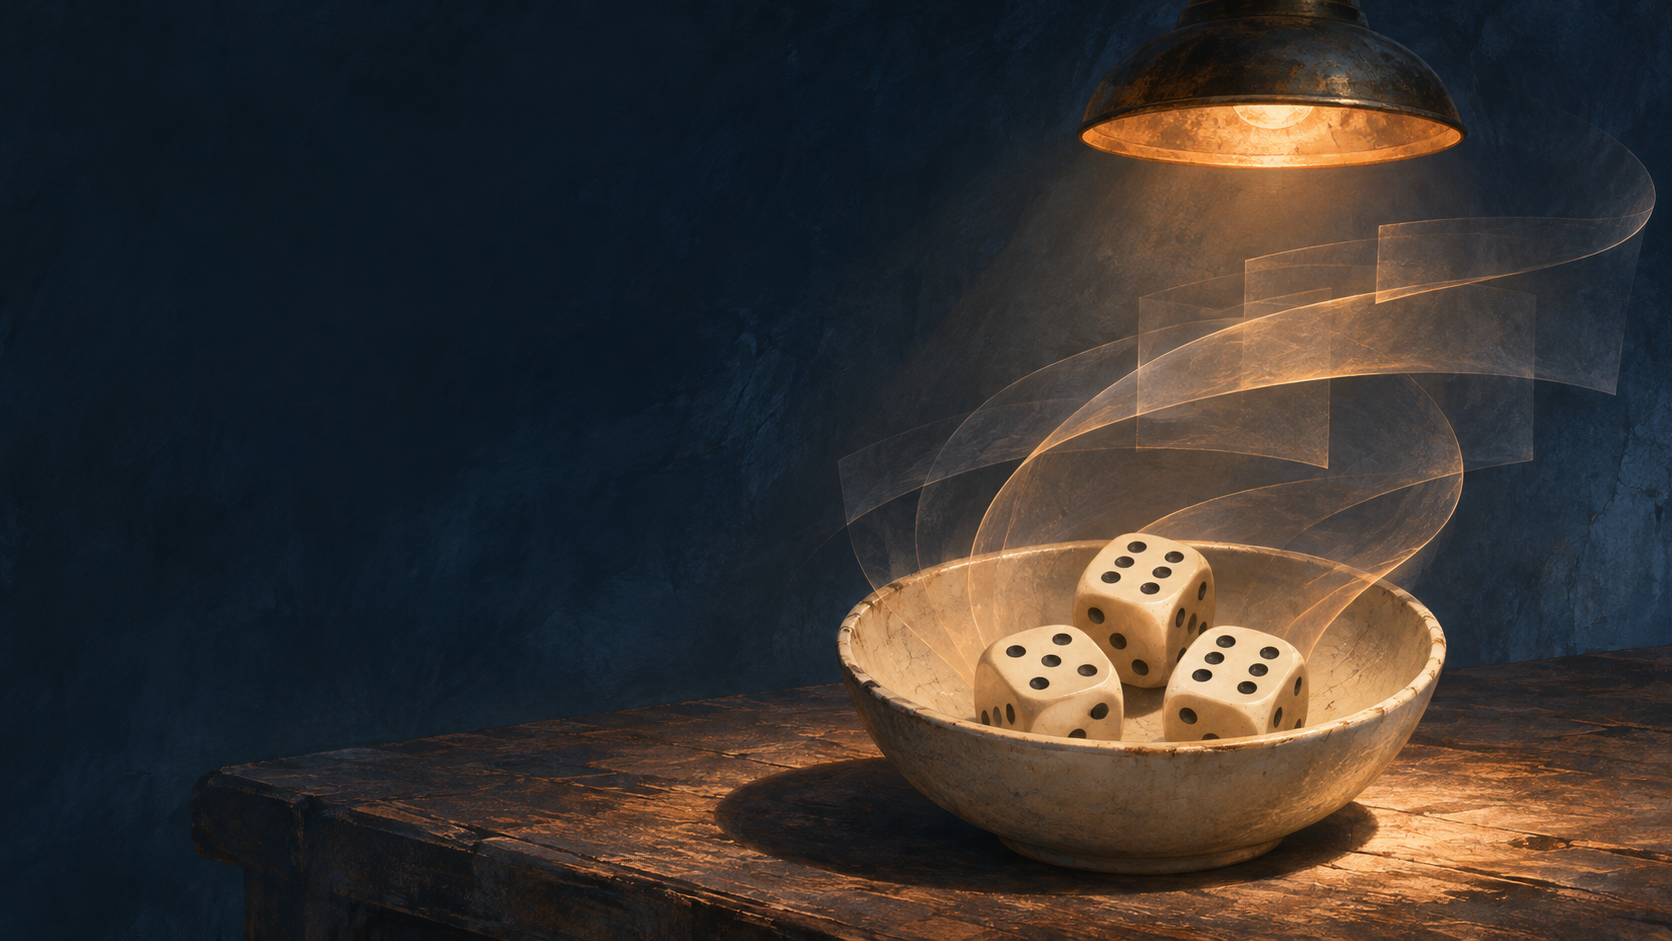
\includegraphics[width=\textwidth]{figures/B01/kaiji_b01_editorial_cover.png}\par
\vspace{3mm}
{\small\color{gray} 扉絵：地下の賽から立ち上がる証拠\par}
\vspace{10mm}
\begin{minipage}{0.960\textwidth}
\textbf{概要}\par
直接観測できない状態や指標を、観測可能な記録と仮定から推定し、予測の妥当性を検証する方法を検討する。
『カイジ』の地下チンチロの二値観測によるベイズ推定を出発点に、局面などの外的要因、観測間の依存関係、潜在状態の変化へ考察を広げる。
賽のモデルでは、尤度、役分布、純損益期待値、逐次判定の誤警報上界と検知時刻を導く。事前確率0.100・判定閾値0.990では、期間無制限の誤警報上界は$1/891$（約0.112\%）である。
理解度推定を応用例とし、ベイズ知識追跡（Bayesian Knowledge Tracing; BKT）では、同じ8回答への尤度がほぼ等しくても習得確率が0.984と0.369に分かれる例を厳密計算する。将来回答によるモデル比較と、履歴・出題条件を含む正答予測の逐次監視を示す。
不確かさの発生源と因果効果の識別条件を整理し、大規模言語モデル（LLM）の品質管理などへの応用・実証計画を検討する。見えない対象の推定を継続して確かめる手順を示し、他分野への応用の見通しを得る。
\end{minipage}
\vfill
{\small 2026年11月6日改訂・フルペーパー版\par}
\end{titlepage}
\pagenumbering{roman}
{\small\setlength{\parskip}{0pt}\tableofcontents}
\clearpage
{\small\setlength{\parskip}{0pt}\listoffigures}
\clearpage
\pagenumbering{arabic}


\section{目的、観測単位、仮定}
\subsection{地下チンチロを足場に、見えない状態の推定へ}
本稿は、直接観測できない状態や指標を観測可能な情報から推定する方法と、その実社会への応用可能性を検討する。出発点とするのは、『カイジ』の地下チンチロに登場する通常賽と456賽を題材とした、二項モデルに基づくベイズ推定である。出目という具体的な記録から、直接には分からない賽の使用戦略を推定する題材は、物語を通じた導入であると同時に、生成規則を明示して推論を検証する基盤となる。

単一賽の二値観測から始め、局面に応じた使用率、3個一式で共有される種類、振り直しの条件へモデルを広げると、同じ見かけの結果でも証拠の強さは変わる。三好の記録とカイジの着眼点を、観測情報を保存する役割と、比較すべき仮説を構成する役割として捉える。条件ごとの尤度から更新量を定めることが、単純なモデルから条件を考慮した推論へ進む道筋となる。
\footnote{フィクションの設定や出来事を、確率計算やシミュレーションで数理的に考察する国内の公開例も見られる\cite{mike2014,nemuru2020}。これらは題材に関する公開Web上の考察例であり、本稿の数式と逐次保証は以下で独立に導出・検証する。}

この推論を他の対象へ移す具体例として、学習時の理解度推定を扱う。正誤だけでは分かりにくい状態を、出題条件や自信度・解答時間等の情報と合わせてどう推定するかが、実務上の動機にある。本稿ではまずBKTの基本形を用い、観測への当てはまり、潜在状態の推定、次回正答の予測を区別する。自信度等を追加した際の精度向上は、今後の検証課題とする。

ここで数値化する対象を区別しておく。正誤や解答時間は観測記録、習得状態はモデルに置く潜在変数、習得確率は観測と仮定から得る推定量である。推定した習得確率が、現実の理解度を直接測定した値になるとは限らない。支援終了等の判断に使う閾値や損失も、状態推定そのものとは別に定める。状態・パラメータの不確かさ、近似計算の誤差、モデル・測定・選択のずれを分けて評価し、将来の観測で妥当性を確かめる。

読み方の案内として、賽の分布・尤度・期待値の導出は第2〜10節、逐次保証と検知は第11〜12節に置いた。理解度推定を主に読む場合は第\ref{sec:bkt}節の更新式と有限標本の曖昧さ、第\ref{sec:calibration}節の予測監視を起点に、保証の基礎を第\ref{sec:performance}節、不確かさの整理を第\ref{sec:uncertainty}節で参照できる。後半では、学習支援、LLMの品質管理、介入の因果効果を扱う際の条件を検討し、計算済みの結果と今後の実証計画を分けて示す。

\subsection{班長の使い分け、三好の記録、カイジの違和感}
地下チンチロを確率の題材として読む際に注目したいのは、
大槻班長による賽の使い分け、三好による出目や勝ち分の記録、
そしてその記録から勝負どころでの強さに違和感を見いだすカイジ、というつながりである\cite{kaiji}。
その周囲には、「ざわざわ」と勝負の行方を見守る人々もいる。
本稿では、班長を「強い人」と見る観戦者の視点も、物語を読むための対比として置く。
通常時には負け、勝負どころでも必ず勝つわけではない相手に対して、
強さへの驚きが、そのまま仕掛けへの疑いになるとは限らない。
通常の勝負を交えながら利益を積み重ねる相手を、
単に「全体でよく勝つ」という印象だけで評価してよいのだろうか。
賭け金が大きいときだけ出目の分布が変わるなら、勝率の集計に加えて、
いつ、どの賭け金で、どの出目が出たかという対応関係が手掛かりになる。

この題材を使う狙いは、違和感を観測と仮説比較の言葉で説明することである。
班長の行動は生成モデル、三好の記録は観測データ、カイジの着眼点は比較すべき仮説に対応する。
記録を取り続けたことによって、局面と出目の関係を後から検討できる点に意味がある。
ただし、本稿の事後確率は登場人物の心理を数値的に再現したものではなく、
仮説と事前確率を明示した観測者にとっての推論である。
原作の全対局を数値データとして復元したわけではないため、
後述の局面別の図は原作の発想に沿った仮想系列として提示する。

\subsection{「強い」「違和感がある」「仕掛けを疑う」を分ける}
同じ勝敗を目にしても、注意を向ける情報と、候補にする説明は人によって異なり得る。
勝ち負けだけが印象に残る観戦者、賭け金と出目を対応させて見る観察者、
仕掛けを知って過去の場面を読み返す読者を、次のように区別する。
これは登場人物や読者を測定して分類した結果ではなく、本稿の説明に用いる視点の整理である。

\begin{center}
\small
\begin{tabular}{p{30mm}p{53mm}p{60mm}}
\toprule
視点 & 注目する情報 & 問いの形\\
\midrule
周囲の観戦者 & 勝敗の印象、班長の強さ & 強い相手だという驚きは、何を手掛かりに違和感へ変わるか。\\
疑い始めた観察者 & 出目、賭け金、局面、記録の対応 & 通常賽だけと、局面に応じて使い分ける戦略のどちらが記録を説明するか。\\
仕掛けを知る再読者 & 過去の場面と、後から得た知識 & その時点までの情報だけでも気付けたか。後の知識を混ぜていないか。\\
\bottomrule
\end{tabular}
\end{center}

「違和感を覚える」という心理反応と、「イカサマ戦略仮説を支持する」という仮説比較は別の対象である。
例えば$A_t$を違和感を自覚したという反応とすれば、その発生率を求めるには、
注意の向け方、提示された情報、本人の回答などの心理・行動データが必要になる。
本稿の$p_t=P(H_1\mid D_{1:t})$は、仮説と観測を明示した計算であり、$P(A_t=1\mid D_t)$を測定した値ではない。
「気付かない人」を機械的に$p_0=0$と置くことも避ける。
仕掛けが説明の候補に入っていない状態と、候補には入るが事前確率が小さい状態は異なる。
通常のベイズ更新では、最初に確率0を置いた仮説は、尤度が有限なデータだけでは復活しない。
新しい仕掛けを知った時点で仮説の候補を広げる問題は、固定した2仮説間の更新から分けて考える。

仕掛けを知って原作を読み返すと、記録の意味を捉え直せる。
一方で、結果の知識が過去の判断を変える後知恵バイアスもある\cite{fischhoff1975}。
本稿では各時点までの情報で進める推論と、仕掛けを知った後の解釈を分ける。
この違いは、第\ref{sec:frequency}節で仮説の発見と判定を分ける心理学的な実験案につなげる。

\subsection{実物の仕掛けから確率モデルへ}
456賽は、出目を4・5・6に限定する仕掛けを持つ賽である。
参考写真を図\ref{fig:photo}に示す。身近な実物を入口にすると、
「低い目が出ない」ことが、強い役の出やすさ、敗北確率、観測時の証拠にどう結びつくかを考えやすい。
写真は仕組みを説明する資料であり、実物の転がり方や確率の一様性を測定したデータではない。
以下では通常賽の1〜6が各$1/6$、456賽の4・5・6が各$1/3$と仮定する。

\begin{center}
\begin{minipage}{0.740\linewidth}
\centering
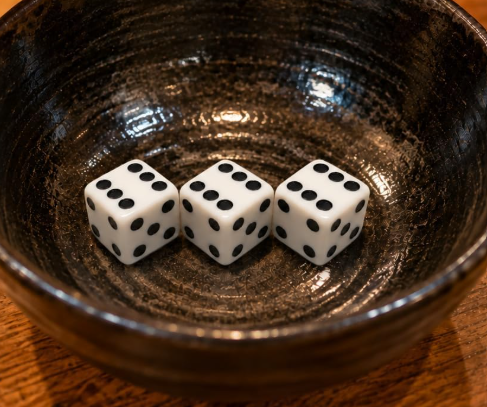
\includegraphics[width=90mm]{figures/P01/kaiji_p01_reference_dice.png}\par
\vspace{4pt}
{\small\raggedright
\refstepcounter{figure}\label{fig:photo}
\addcontentsline{lof}{figure}{\protect\numberline{\thefigure}456賽の参考写真}
\textbf{図\thefigure}\enspace 456賽の参考写真（提供画像）。写真の見え方と、各出目が等確率で出るというモデルの仮定を区別する。\par}
\end{minipage}
\end{center}

\subsection{何の確率を求めるか}
福本伸行『賭博破戒録カイジ』の地下チンチロに登場する456賽を題材とする。
\footnote{公開ルールの参照先は777TOWN.net「帝愛カジノ：対局ルールと役一覧」
（2026年11月3日確認）、\url{https://www.777town.net/casino/chinchirorin/rule.jsp}。
3個の賽・最大3投・親の総取りなし等を記載した同サービスの運営資料であり、
原作そのものの一次資料ではない。本稿の仮定と原作の一致を保証するものではなく、
配当画像の内容は今回の計算に用いていない。}
本稿でいう「疑いの強さ」は、定義した2仮説の間での事後確率である。
実際の人間が疑い始める心理的確率や、不正一般の発生確率を実測するモデルではない。
仮説の候補を変えれば事後確率も変わるため、結論はモデルの範囲とともに示す。

\begin{center}
\begin{tabular}{ll}
\toprule
単位 & 定義\\
\midrule
1個の出目 & 単一賽のHi/Loモデルの観測単位\\
1投 & 同じ種類の賽3個を同時に振る\\
1手番 & 役が成立するまで最大3投する\\
1対戦 & 親と子1人の最終役を比較して精算する\\
\bottomrule
\end{tabular}
\end{center}

\subsection{基本となる設定}
通常賽は1〜6が各$1/6$、456賽は4・5・6が各$1/3$で出ると仮定する。
使用する種類が決まっているとき、3個の賽の出目および別の投の出目は独立とする。
ただし、種類が未知のまま混合した分布では、同じ一式に属する出目を独立とはみなさない。

基準値は、事前確率$p_0=0.100$、456賽使用率$\eta=0.900$である。
これらの数値、一様性、独立性、持ち替え時点は本稿の説明用仮定であり、
原作の実測値や確定設定とは区別する。丼から賽がこぼれる事象は今回除外する。
手番モデルでは、手番開始時に一式を選び、その手番の振り直し中は維持する。

本稿の小数表示は小数点以下3桁へ四捨五入して統一する。これは有効数字3桁とは異なる。
回数・通り数は整数、厳密な値は分数で保持し、計算内部の精度は落とさない。
百分率も小数点以下3桁とする。丸めて$1.000$または$100.000\%$と表示されても、
厳密に確率1であることを意味しない。1との差が小さい場合は、補数を科学表記で併記する。

\begin{center}
\begin{tabular}{ll}
\toprule
記号 & 意味\\
\midrule
$p_t$ & 観測$t$回後の$H_1$の事後確率\\
$p_0$ & 観測開始前の事前確率\\
$\eta$ & $H_1$における456賽の使用率\\
$h,l$ & HiとLoの観測回数\\
$O_t$ & $H_1$対$H_0$の事後オッズ\\
$\theta$ & 判定に使う事後確率の閾値\\
$q$ & 1投で目なしになる確率\\
$G$ & 賭け金1単位に対する1対戦の純損益\\
\bottomrule
\end{tabular}
\end{center}

以下で用いる観測単位の関係を図\ref{fig:a01}に示す。単一賽の出目、1投、1手番、1対戦を区別して読み進める。

\articlefigure{figures/A01/kaiji_a01_observation_units.pdf}{観測単位の整理}{単一賽の出目、3個を同時に振る1投、目なしの振り直しを含む1手番、親と子の最終役を比較する1対戦を区別する。}{fig:a01}{0mm 0mm 0mm 0mm}

\section{単一賽の分布と固定回数の検定}
\subsection{出目の期待値}
通常賽を$X_F$、456賽を$X_{456}$とする。
\begin{align}
P(X_F=k)&=\frac16 \quad(k=1,\ldots,6),\\
P(X_{456}=k)&=
\begin{cases}
1/3 & k\in\{4,5,6\},\\
0 & k\in\{1,2,3\}.
\end{cases}
\end{align}
離散確率変数の期待値$E[X]=\sum_k kP(X=k)$から、
\begin{align}
E[X_F]&=\frac{1+2+3+4+5+6}{6}=\frac{21}{6}=3.500,\\
E[X_{456}]&=\frac{4+5+6}{3}=\frac{15}{3}=5.000.
\end{align}
差は1.500であるが、これらは出目の平均である。
チンチロでは出目から役を作り、相手の役と比較して配当が決まるため、
この差をそのまま勝率や金銭的な利益へ読み替えることはできない。

両分布と出目の平均を図\ref{fig:a02}に示す。

\inlinearticlefigure{figures/A02/kaiji_a02_die_distributions.pdf}{単一賽の分布と出目の平均}{通常賽は1〜6が各1/6、456賽は4・5・6が各1/3となる。出目の平均3.500と5.000は、ゲームの純損益期待値とは異なる。}{fig:a02}{0mm 0mm 0mm 0mm}

\subsection{Hiとシゴロの役を区別する}
単一賽が4以上なら$\HH$、3以下なら$\LL$とする。
したがって、
\[
P(\HH\mid F)=P(\LL\mid F)=\frac12,\qquad
P(\HH\mid456)=1,\quad P(\LL\mid456)=0.
\]
ここでのHiは1個の賽の分類であり、3個に4・5・6が1個ずつ出るシゴロの役とは異なる。

\subsection{全回Hiだったときのp値}
観測の開始点と回数$n$を事前に固定し、Hiの個数を$K$とする。
通常賽の仮説では、
\begin{equation}
K\sim\operatorname{Binomial}(n,1/2),\qquad
P(K=k\mid F)=\binom nk2^{-n}.
\end{equation}
Hiの多い方向を対立仮説とする片側検定で、$K=n$を観測した場合、
\begin{equation}
p_{\mathrm{value}}
=P(K\ge n\mid F)
=P(K=n\mid F)
=2^{-n}.
\end{equation}
$n=7$なら$1/128\simeq0.008<0.010$となる。
これは「通常賽のもとで、観測結果以上にHiへ偏る確率」であり、
$P(F\mid\text{観測})$ではない。
長い系列から都合のよい7連続だけを抽出したり、窓をずらして繰り返し検定したりする場合、
この値を監視全体の誤検出率として使うことはできない。

\section{逐次ベイズ更新の導出}
\subsection{履歴を条件に含める}
導入では$H_0$を「常に通常賽」、$H_1$を「常に456賽」とする。
観測を$D_t\in\{\HH,\LL\}$、過去を$D_{1:t-1}$と書き、
\begin{equation}
p_{t-1}=P(H_1\mid D_{1:t-1})
\end{equation}
と定義する。観測前は$D_{1:0}$が空なので$p_0$が事前確率である。

仮説を固定すると観測間は独立という仮定から、
\begin{equation}
P(D_t\mid H_i,D_{1:t-1})=P(D_t\mid H_i)=\ell_i(D_t).
\end{equation}
全確率の公式を使うと、新しい観測の予測確率は、
\begin{align}
P(D_t\mid D_{1:t-1})
&=\sum_{i=0}^{1}P(D_t\mid H_i,D_{1:t-1})
                         P(H_i\mid D_{1:t-1})\\
&=\ell_1(D_t)p_{t-1}+\ell_0(D_t)(1-p_{t-1}).
\end{align}
これをベイズの定理の分母に代入すれば、
\begin{equation}
\boxed{
p_t=
\frac{\ell_1(D_t)p_{t-1}}
{\ell_1(D_t)p_{t-1}+\ell_0(D_t)(1-p_{t-1})}
}
\label{eq:update}
\end{equation}
を得る。分母は新しい観測の周辺尤度であり、2仮説の重みの和を1に正規化する。
この操作が「前回の事後確率を次回の事前確率にする」という逐次更新である。

\subsection{オッズなら尤度比を掛けるだけになる}
式\eqref{eq:update}と同じ分母を使えば、
\[
1-p_t=
\frac{\ell_0(D_t)(1-p_{t-1})}
{\ell_1(D_t)p_{t-1}+\ell_0(D_t)(1-p_{t-1})}.
\]
両式の比を取ると、共通の分母が消える。
\begin{align}
O_t:=\frac{p_t}{1-p_t}
&=\frac{\ell_1(D_t)p_{t-1}}{\ell_0(D_t)(1-p_{t-1})}\\
&=\underbrace{\frac{p_{t-1}}{1-p_{t-1}}}_{O_{t-1}}
  \underbrace{\frac{\ell_1(D_t)}{\ell_0(D_t)}}_{B_t}.
\end{align}
$B_t$はその観測のベイズ因子（尤度比）である。
有限で正の尤度に対して、$B_t>1$なら$H_1$を支持し、$B_t<1$なら$H_0$を支持する。
反復すると、
\begin{equation}
O_n=O_0\prod_{t=1}^{n}B_t,\qquad p_n=\frac{O_n}{1+O_n}.
\label{eq:odds}
\end{equation}
確率の差を毎回足すのではなく、仮説を支持する比率を積み重ねている。

Hiを1回観測する際の未正規化の重みと正規化を、図\ref{fig:a03}にまとめる。

\articlefigure{figures/A03/kaiji_a03_bayes_update.pdf}{ベイズ更新と重みの正規化}{事前確率と尤度を掛けた重み0.100・0.450を予測確率0.550で割る。純粋な456賽仮説の確率は10.000％から約18.182％へ更新される。}{fig:a03}{0mm 0mm 0mm 0mm}

\subsection{純粋モデルの閉形式と数値例}
Hiなら$B_t=1/(1/2)=2$である。全$n$回Hiなら、
\[
O_n=\frac{p_0}{1-p_0}2^n.
\]
式\eqref{eq:odds}を使って確率へ戻すと、
\begin{equation}
\boxed{p_n=\frac{p_0\,2^n}{1-p_0+p_0\,2^n}}.
\end{equation}
例えば$p_0=0.100$からHiを1回観測すると、
\[
p_1=\frac{1\times0.100}{1\times0.100+0.500\times0.900}
=\frac{0.100}{0.550}\simeq0.182.
\]
7回後は$128/137\simeq0.934$である。
同じ観測のp値$1/128$とは、分母も意味も異なる。

Loの尤度は$\ell_1(\LL)=0$なので、この厳密な$H_1$の事後確率は0になる。
以後のHiでも0から復活しない。これは「常に456賽」という仮説に関する結論であり、
通常賽を混ぜる不正など、別の仮説まで否定するものではない。

Hiだけが続く場合の推移を図\ref{fig:a04}に示す。図の0.990は事後確率の閾値であり、信頼水準や誤検出率ではない。

\inlinearticlefigure{figures/A04/kaiji_a04_pure_posterior.pdf}{Hi連続観測による事後確率}{事前確率10.000％からHiを連続観測した純粋モデル。7回後は約93.431％、10回後に初めて99.000％以上となる。横軸0は事前確率。}{fig:a04}{0mm 0mm 0mm 0mm}

\subsection{何回で閾値を超えるか}
$0<p_0<\theta<1$とし、全回Hiのもとで$p_n\ge\theta$となる条件を求める。
確率をオッズへ変換して、
\begin{align}
p_n\ge\theta
&\iff O_n\ge\frac{\theta}{1-\theta}\\
&\iff 2^n\ge\frac{\theta(1-p_0)}{(1-\theta)p_0}.
\end{align}
したがって最小の整数回数は、
\begin{equation}
n_\theta=
\left\lceil
\frac{\log\!\left(\dfrac{\theta(1-p_0)}{(1-\theta)p_0}\right)}
{\log2}
\right\rceil.
\end{equation}
これは全回Hiという条件付きの到達回数であり、ランダムな観測列での平均検知回数ではない。

\begin{center}
\begin{tabular}{rrrr}
\toprule
事前確率 & 純粋モデルのHi 7回後 & 99.000\%到達：純粋 & 99.000\%到達：90.000\%混合\\
\midrule
1.000\% & 56.388\% & 14回 & 15回\\
10.000\% & 93.431\% & 10回 & 11回\\
20.000\% & 96.970\% & 9回 & 10回\\
50.000\% & 99.225\% & 7回 & 8回\\
\bottomrule
\end{tabular}
\end{center}
比較値は説明用の事前確率であり、各数値に心理的属性を付与していない。

同じ観測列に対する事前確率の違いを図\ref{fig:a05}で比較する。

\articlefigure{figures/A05/kaiji_a05_prior_comparison.pdf}{事前確率による違い}{純粋モデルでHiを連続観測した場合の4条件を比較する。表は7回後の事後確率と、初めて99.000％以上になる観測回数を示す。}{fig:a05}{0mm 0mm 0mm 0mm}

\section{通常賽を混ぜる単一賽モデル}
\subsection{潜在変数を周辺化する}
この節では$H_1$を「各観測で確率$\eta$により456賽、それ以外は通常賽を選ぶ」と変更する。
使用種類を表す潜在変数を$Z_t$とし、$Z_t=1$が456賽、$Z_t=0$が通常賽である。
全確率の公式から、
\begin{align}
P(\HH\mid H_1)
&=P(\HH\mid Z_t=1)P(Z_t=1\mid H_1)
 +P(\HH\mid Z_t=0)P(Z_t=0\mid H_1)\\
&=1\cdot\eta+\frac12(1-\eta)=\frac{1+\eta}{2},\\
P(\LL\mid H_1)
&=0\cdot\eta+\frac12(1-\eta)=\frac{1-\eta}{2}.
\end{align}
$\eta=0.900$ならHiが95.000\%、Loが5.000\%である。
通常賽を10.000\%使っても、その通常賽の半分はHiになるため、Loは10.000\%ではない。
使用率$\eta$は推論側も知っている設定であり、未知の使用率をデータから推定してはいない。

\subsection{HiとLoの証拠は非対称である}
通常賽の尤度はいずれも$1/2$なので、
\begin{equation}
B(\HH)=\frac{(1+\eta)/2}{1/2}=1+\eta,\qquad
B(\LL)=\frac{(1-\eta)/2}{1/2}=1-\eta.
\end{equation}
$\eta=0.900$なら、Hiでオッズは1.900倍、Loで0.100倍になる。
Loの低下分をHiで回復するには、
\[
0.100(1.900)^m\ge1
\iff m\ge\frac{\log10}{\log1.900}\simeq3.587
\]
なので、少なくとも4回のHiが必要である。
これはオッズをLoの直前以上に戻すための回数であり、確率に一定量を足す操作ではない。

Hiを$h$回、Loを$l$回観測すると、
\begin{equation}
O_{h,l}=\frac{p_0}{1-p_0}(1+\eta)^h(1-\eta)^l,\qquad
p_{h,l}=\frac{O_{h,l}}{1+O_{h,l}}.
\label{eq:mixedodds}
\end{equation}
積の順序によらないため、最終値は$h,l$だけで決まる。
一方、途中の推移と最初に閾値を超える時点は、どこでLoが出るかに依存する。
基準設定では、Hi10回で約98.553\%、11回で約99.233\%、
Hi10回とLo1回なら約87.200\%である。

\subsection{対数オッズと極限での検算}
$0<\eta<1$、$0<p_0<1$なら、対数オッズは、
\begin{equation}
\log O_{h,l}
=\log\frac{p_0}{1-p_0}
 +h\log(1+\eta)+l\log(1-\eta).
\end{equation}
積が和になるため、各観測が加える証拠量を見通しやすく、長い系列の数値計算にも向く。
全回Hiの閾値到達回数は、純粋モデルの$\log2$を$\log(1+\eta)$へ置き換えて求められる。

$\eta=0$では2仮説の分布が同じになり、ベイズ因子は常に1、事後確率は変わらない。
$\eta=1$では純粋モデルへ戻り、Loの尤度が0になる。
この端点では$\log(1-\eta)$が有限でないため、対数式へ機械的に代入せず、元の尤度で扱う。

保存系列「Hi 2回、Lo 1回、Hi 17回」での挙動を図\ref{fig:a06}に示す。これは各観測で賽の種類を独立に選ぶ導入用の例であり、次節の3個一式のモデルとは区別する。

\articlefigure{figures/A06/kaiji_a06_mixed_single_die.pdf}{単一賽混合モデルの非対称な証拠}{Hiはオッズを1.900倍、Loは0.100倍にする。3回目のLoの後にHiが4回続くとLo直前の水準を上回る。保存された1系列の例示。}{fig:a06}{0mm 0mm 0mm 0mm}

\section{3個一式を選ぶ場合の尤度}
\subsection{具体的な出目と、全個体Hiという事象}
1投の順序付き出目を$\mathbf{x}=(x_1,x_2,x_3)$とする。
使用種類を固定した条件のもとでは独立なので、
\begin{equation}
\PF(\mathbf{x})=\left(\frac16\right)^3=\frac1{216},\qquad
\PR(\mathbf{x})=\mathbf{1}_{\{x_1,x_2,x_3\ge4\}}\frac1{27}.
\end{equation}
$\mathbf{1}$は条件が成立すると1、それ以外で0となる指示関数である。
一式の選択を周辺化すると、
\begin{equation}
P(\mathbf{x}\mid H_1)
=\eta\PR(\mathbf{x})+(1-\eta)\PF(\mathbf{x}).
\end{equation}
したがって、具体的な出目のベイズ因子は、
\begin{equation}
B(\mathbf{x})=
\begin{cases}
\eta(216/27)+(1-\eta)=1+7\eta & \text{全個体Hi},\\
1-\eta & \text{Loを1個以上含む}.
\end{cases}
\end{equation}
$\eta=0.900$では7.300と0.100である。
4・5・6の内部の値によって比率は変わらないため、この1投の仮説比較では
「全個体Hiかどうか」へ集約しても情報は失われない。

全個体Hiという事象$A$の確率を直接計算しても、
\[
P(A\mid H_0)=\frac{27}{216}=\frac18,\qquad
P(A\mid H_1)=\eta+\frac{1-\eta}{8}
\]
より、同じ尤度比$1+7\eta$が得られる。
ただし、具体的な出目1通りの確率$1/216$と、
27通りからなる事象の確率$1/8$は異なる量である。

\subsection{条件付き独立と周辺の依存関係}
各賽のHi指示変数を$Y_i=\mathbf{1}_{\{X_i\ge4\}}$とする。
一式の種類$Z$が分かれば$Y_1,Y_2,Y_3$は独立であるが、
種類が未知のまま平均すると、
\begin{align}
E[Y_i\mid H_1]&=\eta+\frac{1-\eta}{2}=\frac{1+\eta}{2},\\
E[Y_iY_j\mid H_1]&=\eta+\frac{1-\eta}{4}=\frac{1+3\eta}{4}
\qquad(i\ne j).
\end{align}
ゆえに、
\begin{align}
\operatorname{Cov}(Y_i,Y_j\mid H_1)
&=E[Y_iY_j\mid H_1]-E[Y_i\mid H_1]E[Y_j\mid H_1]\\
&=\frac{1+3\eta-(1+\eta)^2}{4}
=\frac{\eta(1-\eta)}4.
\end{align}
$0<\eta<1$では共分散が正であり、同じ潜在状態を共有することによって依存関係が生じる。
特に$\eta=0.900$では、全個体Hiの確率は$0.900+0.100/8\simeq0.913$であり、
各賽の周辺Hi確率を掛けた$0.950^3\simeq0.857$とは一致しない。

全個体Hiが続く場合、1投ごとのオッズ倍率は7.300である。
単一賽として独立に3回更新した$1.900^3=6.859$を使わないことが重要である。

共通の種類を共有するモデルと、賽ごとの独立選択という別モデルを図\ref{fig:a07}で比較する。

\articlefigure{figures/A07/kaiji_a07_shared_dice_state.pdf}{共通の種類が生む依存関係}{条件付き独立と周辺の独立性は異なる。全個体Hiの確率は共有モデルで0.913、独立選択モデルで0.857となり、共有モデルの共分散は0.023。}{fig:a07}{0mm 0mm 0mm 0mm}

\section{振り直しを含む1手番の尤度}
\subsection{同じ一式を維持するモデル}
手番開始時に$Z$を1回選び、その手番の振り直し中は維持する。
手番間では独立に選ぶ。観測データは各手番の全投擲履歴とする。
有効な手番を$T=(\mathbf{x}_1,\ldots,\mathbf{x}_m)$、$1\le m\le3$と書く。
途中の投はすべて目なしで、最後は役成立、または3投目の目なしで停止する。

使用種類が固定されている条件では各投は独立なので、
\begin{equation}
P(T\mid Z=0)=\prod_{j=1}^{m}\PF(\mathbf{x}_j),\qquad
P(T\mid Z=1)=\prod_{j=1}^{m}\PR(\mathbf{x}_j).
\end{equation}
この有効な手番に対して種類を周辺化すると、
\begin{equation}
\boxed{
P(T\mid H_1)
=\eta\prod_{j=1}^{m}\PR(\mathbf{x}_j)
 +(1-\eta)\prod_{j=1}^{m}\PF(\mathbf{x}_j)
}.
\label{eq:turn}
\end{equation}
停止規則は両仮説で共通であり、観測された履歴から決まる。
有効でない手番の確率は0とする。手番数$m$だけを観測した条件付き尤度ではなく、
出目と停止時点を合わせて観測した確率である。

もし毎投ごとに種類を選び直すなら、
\begin{equation}
\prod_{j=1}^{m}
\left\{\eta\PR(\mathbf{x}_j)+(1-\eta)\PF(\mathbf{x}_j)\right\}
\end{equation}
となるが、これは別の生成モデルである。
積と混合の順序を入れ替えると、潜在状態が共有される範囲まで変わってしまう。

\subsection{振り直しが持つ証拠}
456賽の3出目は、すべて同じならゾロ目、2個同じなら通常の目、
すべて異なれば4・5・6のシゴロとなる。
したがって目なしが存在せず、456賽を選んだ手番は必ず1投で終了する。
振り直しが観測された手番では$\PR(T)=0$となり、
\[
\frac{P(T\mid H_1)}{P(T\mid H_0)}
=\frac{(1-\eta)\PF(T)}{\PF(T)}=1-\eta.
\]
このとき、その手番に通常賽が使われたことは分かるが、
通常賽を混ぜる戦略$H_1$全体の可能性は0にはならない。
なお、通常賽一式を選んでもHiだけの1投で終わることはあるため、
1投で全個体Hiだったという観測だけで、その投の使用種類が確定するわけではない。

停止規則を図\ref{fig:a08}に示す。図では使用種類を固定し、$q$を1投の目なし確率、$a_r$を特定の成立役$r$の1投の確率とする。最終役分布の導出は第\ref{sec:final}節で詳述する。

\articlefigure{figures/A08/kaiji_a08_turn_stopping_tree.pdf}{最大3投の手番の停止木}{目なしだけを振り直し、3投目は目なしでも終了する。通常賽で3投目に役が成立する確率は1/8、3投目まで振る確率は1/4。平均投数は1.750回。}{fig:a08}{0mm 0mm 0mm 0mm}

\subsection{勝負どころで一式を選ぶ局面別モデル}\label{sec:context}
これまでの$H_1$は、各手番で一定確率$\eta$により456賽を選ぶ仮説だった。
導入の問題意識に合わせ、手番$t$の結果が出る前に分かる局面を$C_t$とし、
使用率を$\eta(C_t)$へ拡張する。$C_t$には賭け金、親番、事前に定義した機会などを用いる。
出目を見てから「勝負どころ」を選ぶ操作は、この設定に含めない。

比較する帰無仮説$H_0$は常に通常賽を使う仮説である。
局面別の戦略仮説を$H_{1,C}$とすると、全投擲履歴$T_t$の尤度は、
\begin{equation}
P(T_t\mid H_{1,C},C_t)
=\eta(C_t)P_{456}(T_t)+\{1-\eta(C_t)\}P_F(T_t).
\end{equation}
事前に固定した局面列に条件付け、手番間で一式を独立に選ぶなら、
各手番のベイズ因子とオッズ更新は、
\begin{align}
B_t(C_t)&=1+\eta(C_t)\left\{\frac{P_{456}(T_t)}{P_F(T_t)}-1\right\},\\
O_t&=O_{t-1}B_t(C_t),\qquad p_t=\frac{O_t}{1+O_t}.
\end{align}
局面が過去の履歴から適応的に決まる場合は、その履歴も条件に含める必要がある。
本版の数値例では、局面列をすべて観測前に固定している。

通常時の使用率を$\eta(C_t)=0$とすれば、両仮説とも通常賽を予測するため$B_t=1$である。
通常時にLoや負けを観測しても、それだけでは局面別仮説に対する疑いは下がらない。
一方、一定使用率の仮説ではLoがその仮説に不利な証拠となる。
平打ちが疑いを下げるかどうかは、何を予測する仮説と比較するかによって異なる。

\clearpage
\subsection{賭け金・勝敗・全投擲履歴を対応させた仮想系列}
図\ref{fig:a14}は、原作の対局記録そのものではなく、固定した乱数種で生成した20手番の例である。
4・8・12・16・20手番を観測前に勝負どころと決め、賭け金を10単位、
その他の15手番を1単位とする。通常時は$\eta=0$、勝負どころでは$\eta=0.900$とした。
賭け金は説明用の相対単位であり、原作のペリカ額を復元したものではない。
各手番で一式を選び、目なしだけを振り直して最大3投で止める。
相手は独立な通常賽で同様に手番を完了する。
勝敗には後述の順位A（ピンゾロが最上位、2〜6のゾロ目は同格）を用いる。

局面を使わない比較用の仮説$H_{1,G}$では、同じ予定表における平均使用率
\[
\bar\eta=\frac{5\times0.900+15\times0}{20}=\frac9{40}=0.225
\]
を全手番に一律に使う。$H_0$と事前確率$p_0=0.100$は共通であるが、
$H_{1,C}$と$H_{1,G}$は異なる対立仮説である。2曲線は同じ仮説の信頼区間や誤差帯ではない。

この保存系列では、通常時は9勝6敗0分、勝負どころは4勝1敗0分となった。
実行設定IDは\texttt{CTX20-v1}で、被観測者の乱数種は20261103、相手は20261108である。
後述の\texttt{CONST20-v1}とは生成設定が異なるため、同じ乱数種でも出目列は一致しない。
相手の系列は勝負どころの敗戦も含む挙動を説明するための例示として選んだもので、頻度推定には用いない。
8手番目は被観測者のシゴロが相手の444に負ける。それでも被観測者の出目は全個体Hiであり、
通常賽と456賽の比較では使用戦略を支持する証拠となる。観戦者の勝敗の印象と、出目の尤度による判断は区別する。
勝負どころの5手番はすべて全個体Hiで終わるため、局面別のベイズ因子は各7.300となる。
通常時のベイズ因子は1なので、20手番後は、
\[
p_{20}^{C}=\frac{0.100(7.300)^5}{0.900+0.100(7.300)^5}\simeq1.000.
\]
ただし$1-p_{20}^{C}\simeq4.340\times10^{-4}>0$であり、丸め表示が1になっただけである。
同じ系列の全個体Hiは4・8・11・12・16・18・20手番の7回、残り13回はLoを含む。
一定使用率$\bar\eta=9/40$の仮説では、
\[
M_{20,G}=\left(\frac{103}{40}\right)^7\left(\frac{31}{40}\right)^{13},\qquad
p_{20}^{G}=\frac{M_{20,G}}{9+M_{20,G}}\simeq0.752.
\]
したがってこの終点も、本文の回数から独立に再計算できる。
この差は、局面と出目の対応を仮説に含めたことによる例示であり、
局面別モデルが常に優れることや、検知率・誤警報率を評価した結果ではない。

推定には被観測者の全投擲履歴と事前に定まる局面を用い、生成時の賽の種類は使わない。
相手の分布は両仮説で同じなので、相手の記録の尤度は比で相殺される。
また、双方の出目から決まる勝敗を全投擲履歴と独立な追加観測として掛け合わせると、
同じ情報を二重に数える。勝敗の段は記録の読み取りを助ける表示である。
金額の収支は配当倍率に依存するため、本図では勝敗と賭け金までを示す。
整数の手番軸、全記録、ベイズ因子は再実行用ソースとCSV・JSONに保存した。

\articlefigure{figures/A14/kaiji_a14_context_strategy.pdf}{勝負どころでの使い分けと記録}{事前に決めた賭け金、通常賽の相手に対する勝敗、2種類の対立仮説の事後確率を対応させた仮想系列。通常時は局面別モデルのベイズ因子が1となり、疑いが横ばいになる。原作の実対局記録の復元や検知性能の評価ではない。}{fig:a14}{0mm 0mm 0mm 0mm}

\section{1投の役確率を組合せから求める}
\subsection{通常賽216通りの分類}
順序付き出目の総数は$6^3=216$通りである。
ピンゾロは$(1,1,1)$の1通り、その他のゾロ目は2〜6の5通りである。
シゴロとヒフミは、それぞれ異なる3数字の並べ替えなので$3!=6$通りずつになる。

通常の目$k$は、2個の同じ数字$a$と、残りの数字$k$で決まる。
$a\ne k$の選び方が5通り、$k$を置く位置が3通りなので、
\begin{equation}
N_F(\text{$k$の目})=(6-1)\binom31=5\times3=15.
\end{equation}
6種類の通常の目の合計は$6\times15=90$通りとなる。

3個とも異なる出目は$\binom63\,3!=120$通りである。
このうちシゴロとヒフミを除いたものが、振り直し対象の目なしだから、
\begin{equation}
N_F(\text{目なし})=\binom63\,3!-2\cdot3!=120-12=108.
\end{equation}
合計は$1+5+6+90+108+6=216$となり、分類が全体を尽くす。

\subsection{456賽27通りの分類}
出目の総数は$3^3=27$通りである。
ゾロ目は444・555・666の3通り、シゴロは$3!=6$通りである。
通常の目$k\in\{4,5,6\}$については、重複する数字の選び方が2通りなので、
\begin{equation}
N_{456}(\text{$k$の目})=(3-1)\binom31=2\times3=6.
\end{equation}
よって$3+6+3\times6=27$で全体となり、目なしは0通りである。

\begin{center}
\begin{tabular}{lrrrr}
\toprule
役 & 通常賽の通り数 & 通常賽の確率 & 456賽の通り数 & 456賽の確率\\
\midrule
ピンゾロ & 1 & $1/216$ & 0 & 0\\
ゾロ目（2〜6） & 5 & $5/216$ & 3 & $1/9$\\
シゴロ & 6 & $1/36$ & 6 & $2/9$\\
4・5・6の目 & 各15 & 各$5/72$ & 各6 & 各$2/9$\\
1・2・3の目 & 各15 & 各$5/72$ & 0 & 0\\
目なし & 108 & $1/2$ & 0 & 0\\
ヒフミ & 6 & $1/36$ & 0 & 0\\
\midrule
合計 & 216 & 1 & 27 & 1\\
\bottomrule
\end{tabular}
\end{center}

ここでは確率集計のため、ピンゾロ以外のゾロ目をまとめている。
異なるゾロ目間の強弱を採用する場合、損益計算では出目別に分割する必要がある。

全列挙による内訳を図\ref{fig:a09}に示す。分母が異なるので、棒の長さは共通の確率尺度で比較する。

\articlefigure{figures/A09/kaiji_a09_role_combinatorics.pdf}{1投の役の通り数と確率}{順序付き出目216通り・27通りを全列挙した1投の役分布。各行に正確な通り数／全通り数を示し、下段に数え上げの式を添えた。}{fig:a09}{0mm 0mm 0mm 0mm}

\section{最大3投による最終役分布}\label{sec:final}
\subsection{互いに排反な停止経路を足す}
1投の目なし確率を$q$、成立役$r$が出る確率を$a_r$とする。
役$r$で手番が終わる経路は、
\begin{enumerate}
\item 1投目で$r$：確率$a_r$。
\item 1投目が目なし、2投目で$r$：確率$qa_r$。
\item 最初の2投が目なし、3投目で$r$：確率$q^2a_r$。
\end{enumerate}
これらは停止時点が異なり、互いに排反なので、
\begin{equation}
\boxed{
P_{\mathrm{turn}}(r)=a_r+qa_r+q^2a_r=a_r(1+q+q^2)
}.
\end{equation}
3投とも目なしの確率は、
\begin{equation}
P_{\mathrm{turn}}(\mathrm{none})=q^3.
\end{equation}
$q<1$なら有限等比級数を用いて、
\[
P_{\mathrm{turn}}(r)=a_r\frac{1-q^3}{1-q}
\]
とも書ける。全成立役の和が$\sum_r a_r=1-q$であることから、
\begin{equation}
\sum_rP_{\mathrm{turn}}(r)+q^3
=(1-q)(1+q+q^2)+q^3=1
\end{equation}
となり、正規化を確認できる。

通常賽では$q=1/2$なので、成立役は1投の$7/4$倍、最終目なしは$1/8$となる。
例えばシゴロの最終確率は、
\[
\frac1{36}\left(1+\frac12+\frac14\right)=\frac7{144}\simeq0.049.
\]
456賽では$q=0$なので、1投と1手番の分布が一致する。

\begin{center}
\begin{tabular}{lrr}
\toprule
最終役 & 通常賽：最大3投 & 456賽：1投で確定\\
\midrule
ピンゾロ & $7/864$ & 0\\
ゾロ目（2〜6） & $35/864$ & $1/9$\\
シゴロ & $7/144$ & $2/9$\\
4・5・6の目 & 各$35/288$ & 各$2/9$\\
1・2・3の目 & 各$35/288$ & 0\\
目なし & $1/8$ & 0\\
ヒフミ & $7/144$ & 0\\
\bottomrule
\end{tabular}
\end{center}

これは「目なしが出るたびに無制限で振り続ける」モデルではない。
無制限なら成立役の確率は$a_r/(1-q)$へ変わり、最終目なしが残らなくなる。
最大3投では目なし12.500\%が残るため、単に役成立を条件にした分布へ置き換えてはならない。

1投から最終役分布への変化と、通常賽・456賽の比較を図\ref{fig:a10}に示す。

\articlefigure{figures/A10/kaiji_a10_final_role_distribution.pdf}{1投と手番終了時の役分布}{上段は通常賽の振り直しによる変化、下段は通常賽と456賽の最終分布を比較する。各行の分数は正確な確率であり、カテゴリ順は配当順位を意味しない。}{fig:a10}{0mm 3mm 0mm 3mm}

\subsection{平均何投で手番が終わるか}
手番の投数を$M\in\{1,2,3\}$とする。
3投目まで到達したら、3投目に役が出ても出なくても$M=3$なので、
\begin{equation}
P(M=1)=1-q,\quad P(M=2)=q(1-q),\quad P(M=3)=q^2.
\end{equation}
期待値を直接計算すると、
\begin{align}
E[M]&=1(1-q)+2q(1-q)+3q^2\\
&=1+q+q^2.
\end{align}
通常賽では$7/4=1.750$投、456賽では1投である。
手番開始時に一式を選ぶ混合戦略では、
\[
E[M\mid H_1]=\eta\cdot1+(1-\eta)\cdot\frac74.
\]
$\eta=0.900$なら1.075投となる。これは出目平均や損益平均とは別の期待値である。

\subsection{混合戦略と、観測データを捨てた場合の尤度}
手番内で一式を維持するため、最終役の分布は全確率の公式から、
\begin{equation}
P_{\mathrm{turn}}(r\mid H_1)
=\eta P_{\mathrm{turn},456}(r)
 +(1-\eta)P_{\mathrm{turn},F}(r)
\end{equation}
となる。単一投の混合分布を先に作ってから振り直し計算をするのは、
毎投ごとに一式を選び直す別モデルに対応する。

観測を「最終役だけ」にする場合、この最終役分布が尤度になる。
例えばシゴロの役だけを見た場合、$\eta=0.900$でのベイズ因子は、
\begin{align}
B_{\mathrm{final}}(\text{シゴロ})
&=\frac{\eta(2/9)+(1-\eta)(7/144)}{7/144}\\
&=\eta\frac{32}{7}+(1-\eta)
=\frac{59}{14}\simeq4.214.
\end{align}
一方、「1投目がシゴロで終了した」という全履歴を観測した場合は、
\[
B_{\mathrm{full}}=\frac{\eta(2/9)+(1-\eta)(1/36)}{1/36}
=1+7\eta=7.300
\]
となる。最終役が同じでも、何投目に出たかという情報を捨てるかで尤度が変わる。
最終役だけを記録したデータへ、全履歴用の尤度7.300を適用してはならない。

記録する情報に対応する2つの観測事象を図\ref{fig:a11}で比較する。図の尤度はシゴロの6つの順列をまとめた事象の確率である。

\articlefigure{figures/A11/kaiji_a11_retained_observation_information.pdf}{履歴を残すか、最終役だけを残すか}{1投目のシゴロと、投数未記録の最終役シゴロでは、ベイズ因子が7.300と約4.214に分かれる。実際に記録した情報に合わせて尤度を選ぶ。}{fig:a11}{0mm 0mm 0mm 0mm}


\subsection{保存された手番全履歴からの逐次更新例}
実行設定IDは\texttt{CONST20-v1}である。
一定使用率90.000\%の生成であり、局面別の\texttt{CTX20-v1}と区別する。

事前確率$p_0=0.100$、一式の456賽選択率$\eta=0.900$で、
保存された20手番の順序付き全履歴を使う。
各手番$T_t$のベイズ因子を$B_t=P(T_t\mid H_1)/P(T_t\mid H_0)$とすると、
\begin{equation}
\log_{10}O_n=\log_{10}\frac{p_0}{1-p_0}
 +\sum_{t=1}^{n}\log_{10}B_t.
\end{equation}
図\ref{fig:a12}では、上段に事後確率、下段に直接加算した対数オッズを示す。
この保存系列は全手番が1投目で終了しており、
12手番目の$(1,5,1)$だけがLoを含む。他の19手番は全個体Hiである。
したがって$B_{12}=0.100$、他の手番では$B_t=7.300$となる。
最初の4つの事後確率は約0.448、0.856、0.977、0.997である。

11手番後と12手番後の対数オッズは約8.542と7.542となり、
オッズの10分の1への減少が対数軸では1の低下として現れる。
この時点の事後確率はすでに1に極めて近いため、通常の確率軸では低下を判別しにくい。
20手番後でも$1-p_{20}\simeq3.557\times10^{-15}>0$であり、
丸めた表示から事後確率が厳密に1になったと解釈しない。
この例における99.000％への初到達は4手番目だが、平均検知手番数や誤検出率の推定ではない。


保存系列の全20手番を以下に示す。各ベイズ因子は出目の全履歴に対応する尤度比である。

\begin{center}
\small
\renewcommand{\arraystretch}{1.000}
\begin{tabular}{rrr}
\toprule
手番 & 観測した全投擲（各手番1投） & ベイズ因子 $B_t$\\
\midrule
1 & $(4,4,4)$ & $7.300$\\
2 & $(6,4,4)$ & $7.300$\\
3 & $(6,6,6)$ & $7.300$\\
4 & $(4,4,5)$ & $7.300$\\
5 & $(5,6,6)$ & $7.300$\\
6 & $(5,5,6)$ & $7.300$\\
7 & $(5,4,4)$ & $7.300$\\
8 & $(4,4,5)$ & $7.300$\\
9 & $(5,4,4)$ & $7.300$\\
10 & $(4,4,5)$ & $7.300$\\
11 & $(4,6,5)$ & $7.300$\\
12 & $(1,5,1)$ & $0.100$\\
13 & $(5,4,5)$ & $7.300$\\
14 & $(6,6,5)$ & $7.300$\\
15 & $(4,4,6)$ & $7.300$\\
16 & $(5,4,6)$ & $7.300$\\
17 & $(6,5,6)$ & $7.300$\\
18 & $(6,5,4)$ & $7.300$\\
19 & $(4,4,6)$ & $7.300$\\
20 & $(5,5,6)$ & $7.300$\\
\bottomrule
\end{tabular}
\end{center}

\articlefigure{figures/A12/kaiji_a12_turn_posterior.pdf}{手番の全履歴を用いた逐次更新}{12手番目の(1,5,1)でオッズが10分の1になる。対数オッズを併記することで、事後確率が1に近い領域の変化も確認できる。}{fig:a12}{0mm 0mm 0mm 0mm}

\section{勝率と純損益期待値への接続}
\subsection{配当表を明示してから期待値を取る}
親の最終役を$R_P$、子の最終役を$R_C$とする。
2人の出目生成が独立で、親の最終役にかかわらず子も手番を完了すると仮定すれば、
\[
P(R_P=r,R_C=s)=P_P(r)P_C(s).
\]
役の強弱を表す関数を$v(r)$と定めると、
\begin{align}
P(\text{親の勝ち})&=\sum_{r,s}P_P(r)P_C(s)\,
                         \mathbf{1}_{\{v(r)>v(s)\}},\\
P(\text{引き分け})&=\sum_{r,s}P_P(r)P_C(s)\,
                         \mathbf{1}_{\{v(r)=v(s)\}}.
\end{align}
この書き方では、同じ強さなら引き分けとする。親優遇等の規則を採用する場合は勝敗関数を変更する。

賭け金1単位に対する親の純損益表を$g(r,s)$とすれば、
\begin{equation}
\boxed{
E[G]=\sum_{r,s}P_P(r)P_C(s)\,g(r,s)
}.
\label{eq:profit}
\end{equation}
勝ちは正、負けは負、同点で返却される場合は0とする。
役に便宜上付けた番号を平均するのではなく、実際に受け渡す純損益を平均する。
賭け金$b$に比例する配当なら、$E[G_b]=bE[G]$である。

配当表を確定する前に、異なるゾロ目同士の強弱、同点の扱い、
ヒフミと特殊役が同時に出た場合の倍率の組み合わせ等を明文化する。
以下では未確定部分をパラメータとして残し、明示した比較用配当に限って損益の数値例も示す。

\subsection{倍率をパラメータにした期待純損益}
順位Aで、勝者の役により配当倍率が決まり、同格は返却とする比較用の配当族を定義する。
ピンゾロの倍率を$m_P$、2〜6のゾロ目を$m_T$、シゴロを$m_S$、通常の目を$m_D$と置く。
勝者の役が$r$なら、勝ち側は$+m_r$、負け側は$-m_r$となる反対称な損益表である。
敗者のヒフミ倍率をさらに掛ける等の規則は、この配当族には含めない。
目なし・ヒフミが勝者となる組では便宜上$m_D$とするが、456賽側はそれらより強い役しか出さないため、以下の$K$には寄与しない。
双方が独立に手番を完了する条件で、456賽対通常賽の期待純損益は、
\begin{equation}
\boxed{K(m_P,m_T,m_S,m_D)
=-\frac7{864}m_P+\frac{271}{3888}m_T
+\frac{109}{648}m_S+\frac{155}{432}m_D.}
\label{eq:param-payoff}
\end{equation}
これは式\eqref{eq:profit}で、勝つ役の倍率を加算し、負けたときの相手の倍率を減算して集約したものだ。
たとえばピンゾロは自分には出ず、相手の最終確率$7/864$だけが負の係数となる。
各通常目4・5・6の係数は$155/1296$で、3役の合計が$155/432$になる。

\begin{center}
\begin{tabular}{rrrrrl}
\toprule
$m_P$&$m_T$&$m_S$&$m_D$&$K$の厳密値&小数表示\\
\midrule
1&1&1&1&$4577/7776$&0.589\\
5&3&2&1&$2239/2592$&0.864\\
5&5&2&1&$7801/7776$&1.003\\
\bottomrule
\end{tabular}
\end{center}
倍率の行は感度を読むための仮定で、原作の配当を確定した表ではない。
通常賽同士なら、どの行でも反対称性から期待純損益は0になる。
以後、比較用に倍率をすべて1とした場合には$K=4577/7776$を用いる。
原作の規則を確定できれば、一般の$g(r,s)$を入れ替えて再計算できる。

\subsection{通常賽同士の対称性を検算に使う}
同じ役分布$P$を使う2人について、$g(r,s)=-g(s,r)$かつ同点の損益が0なら、
\begin{align}
E[G]&=\sum_{r,s}P(r)P(s)g(r,s)\\
&=\sum_{r,s}P(s)P(r)g(s,r)\\
&=-\sum_{r,s}P(r)P(s)g(r,s)=-E[G].
\end{align}
よって$E[G]=0$である。
通常賽同士の計算が0にならない場合、親優遇、手数料、停止規則の違い、
あるいは損益表・実装の誤りがないかを確認できる。
勝率だけでは引き分けや配当倍率を反映しないため、勝率と損益期待値は別々に示す。

確率と損益表を組み合わせる計算手順、および条件付きの検算式を図\ref{fig:a13}にまとめる。


\subsection{90.000\%混合戦略の期待値はどこまで簡単になるか}
子の分布と賭け金を固定し、手番開始時に親の一式を独立に選ぶ場合、
式\eqref{eq:profit}の線形性から、
\begin{align}
E[G\mid H_1]
&=\sum_{r,s}
\{\eta P_{456}(r)+(1-\eta)P_F(r)\}P_C(s)g(r,s)\\
&=\eta E[G\mid456]+(1-\eta)E[G\mid F].
\end{align}
ここで$P_{456},P_F$はこの節では最終役分布を表す。
子が通常賽で、通常賽同士の損益表が反対称なら$E[G\mid F]=0$なので、
\[
E[G\mid H_1]=0.900E[G\mid456].
\]
この関係は配当の具体値を入れる前にも分かる。
ただし賽の選択が賭け金や相手の状態に依存する戦略では、条件付き分布から計算し直す必要がある。
親番の継続、複数の子、賭け金上限、破産は1対戦の計算から分けて拡張する。



\articlefigure{figures/A13/kaiji_a13_expected_payoff_framework.pdf}{役の確率から純損益期待値へ}{役分布と損益表から純損益期待値を求める枠組み。損益表は未確定の記号表であり、下段の恒等式は明示した条件の下で成り立つ。}{fig:a13}{0mm 4mm 0mm 4mm}


\subsection{456賽の最終役ごとに、負ける確率を求める}\label{sec:conditional-loss}
ここでは金額の配当を入れる前に、勝敗だけに関する思考実験を行う。
自分は456賽、相手は通常賽を使い、両者が独立に最大3投の手番を完了し、
同じ強さなら引き分けとする。親の役によって子が振らずに終わる規則は採用しない。
異なるゾロ目の強弱は未確定なので、比較のために次の2通りを明示的に仮定する。
\begin{description}
\item[順位A：] ピンゾロ $>$ 2〜6のゾロ目（すべて同格） $>$ シゴロ $>$
6の目 $>$ 5の目 $>\cdots>$ 1の目 $>$ 目なし $>$ ヒフミ。
\item[順位B：] ピンゾロ $>$ 666 $>$ 555 $>$ 444 $>$ 333 $>$ 222 $>$
シゴロ $>$ 6の目 $>\cdots>$ 1の目 $>$ 目なし $>$ ヒフミ。
\end{description}
これは感度を比較するための2規則であり、原作の配当・役順位を確定したという意味ではない。
順位Bでは、先の集約表のゾロ目（2〜6）を出目別に分けてから計算する。
各ゾロ目の通常賽での最終確率は$(1/216)(7/4)=7/864$である。

順位を表す$v$を固定すると、自分の最終役$r$が分かった後の敗北確率は、
\begin{equation}
\boxed{L(r)=P(\text{負け}\mid R_{456}=r)
=\sum_s P_F^{\mathrm{final}}(s)\,
\mathbf{1}_{\{v(s)>v(r)\}}.}
\end{equation}
同様に、
\begin{align}
D(r)&=\sum_s P_F^{\mathrm{final}}(s)\,\mathbf{1}_{\{v(s)=v(r)\}},\\
W(r)&=\sum_s P_F^{\mathrm{final}}(s)\,\mathbf{1}_{\{v(s)<v(r)\}},
\end{align}
であり、$W(r)+D(r)+L(r)=1$となる。
条件を付けた後の敗北確率$L(r)$と、その役が出て負ける同時確率
$P_{456}^{\mathrm{final}}(r)L(r)$を区別する。

例えば6の目より強い役は、両順位ともピンゾロ・その他のゾロ目・シゴロなので、
\begin{equation}
L(6\text{の目})
=\frac7{864}+\frac{35}{864}+\frac7{144}
=\frac7{72}\simeq9.722\%.
\end{equation}
5の目なら相手の6の目、4の目なら相手の5・6の目も敗北に加わるため、
\[
L(5\text{の目})=\frac7{72}+\frac{35}{288}=\frac7{32},\qquad
L(4\text{の目})=\frac7{72}+2\frac{35}{288}=\frac{49}{144}.
\]
444で負ける確率は、順位Aではピンゾロだけの$7/864$だが、
順位Bでは555・666も加わり$3(7/864)=7/288$となる。
456賽の27通りは下表の7役に分かれる。同じ役の順序違い等は、この順位では同じ敗北確率となる。

\begin{center}
\small
\begin{tabular}{lrrr}
\toprule
456賽側の最終役 & その役の確率 & 敗北率：順位A & 敗北率：順位B\\
\midrule
444 & $1/27$ & $7/864$（0.810\%） & $7/288$（2.431\%）\\
555 & $1/27$ & $7/864$（0.810\%） & $7/432$（1.620\%）\\
666 & $1/27$ & $7/864$（0.810\%） & $7/864$（0.810\%）\\
シゴロ & $2/9$ & $7/144$（4.861\%） & $7/144$（4.861\%）\\
6の目 & $2/9$ & $7/72$（9.722\%） & $7/72$（9.722\%）\\
5の目 & $2/9$ & $7/32$（21.875\%） & $7/32$（21.875\%）\\
4の目 & $2/9$ & $49/144$（34.028\%） & $49/144$（34.028\%）\\
\bottomrule
\end{tabular}
\end{center}

\articlefigure{figures/A15/kaiji_a15_conditional_loss.pdf}{456賽の役ごとの敗北確率}{通常賽の相手が最大3投で出す最終役と比較した条件付き敗北確率。順位Aは2〜6のゾロ目を同格、順位Bは666から222まで出目順とする。分数は厳密値、百分率は丸め値である。配当を含む損益期待値とは区別する。}{fig:a15}{0mm 0mm 0mm 0mm}

\subsection{役の発生確率で重み付けした勝敗と、使い分けの利益}
役が分かる前の敗北率は、$L(r)$を456賽側の役分布で平均して、
\[
P(\text{負け}\mid456)=\sum_r P_{456}^{\mathrm{final}}(r)L(r)
\]
と求める。順位Aでは、
\begin{align}
P(\text{勝ち}\mid456)&=\frac{967}{1296}\simeq74.614\%,\\
P(\text{引き分け}\mid456)&=\frac{749}{7776}\simeq9.632\%,\\
P(\text{負け}\mid456)&=\frac{1225}{7776}\simeq15.754\%.
\end{align}
順位Bでは順に$647/864$、$721/7776$、$77/486$となり、約74.884\%、9.272\%、15.844\%である。
これらは上記の独立性・停止規則・順位に対する厳密な計算であり、原作の実測勝率ではない。
456賽でも負けるため、単独の敗戦はその手番で通常賽だったことを意味しない。
勝敗だけを観測する場合も、各仮説の勝敗確率から尤度を作る必要がある。

導入の「勝負どころで稼ぐ」という点は、賭け金$b(C)$と使用率$\eta(C)$の結び付きにも現れる。
局面の発生確率を$\pi(C)$、単位賭け金の純損益を$G$とすると、
\begin{equation}
E[G_b]=\sum_C\pi(C)b(C)\left[
\eta(C)E[G\mid456,C]+\{1-\eta(C)\}E[G\mid F,C]\right].
\end{equation}
相手の分布・役順位・配当規則が局面で変わらず、通常賽同士の純損益の期待値が0なら、
\begin{equation}
E[G_b]=E[b(C)\eta(C)]E[G\mid456].
\end{equation}
一般に$E[b\eta]=E[b]E[\eta]+\operatorname{Cov}(b,\eta)$であり、
使用率の平均だけを同じにしても、賭け金との相関によって金額の期待値は変わる。
図\ref{fig:a14}の予定表では$E[b\eta]=9/4=2.250$、
$E[b]E[\eta]=(13/4)(9/40)=117/160\simeq0.731$である。
前者は局面別戦略、後者は同じ平均使用率で賭け金と独立に使う戦略の係数に対応する。
これは説明用の予定表の係数である。式\eqref{eq:param-payoff}の比較用配当なら数値化できるが、
原作のペリカ額を再現するには原作の配当・親番・精算規則を別途確定する必要がある。

\clearpage
\section{ノートブックとの対応と検証範囲}
\begin{center}
\begin{tabular}{ll}
\toprule
関数・処理 & 対応する計算\\
\midrule
\texttt{bayes\_update} & 式\eqref{eq:update}の逐次更新\\
\texttt{single\_die\_history} & 単一賽の連続観測\\
\texttt{turn\_likelihood} & 種類を固定した手番全体の尤度\\
\texttt{update\_turn} & 式\eqref{eq:turn}の混合と更新\\
\texttt{exact\_roll\_distribution} & 216通り・27通りの全列挙\\
\texttt{exact\_turn\_distribution} & 有限等比級数による最終役分布\\
\bottomrule
\end{tabular}
\end{center}

基準設定は事前確率10.000\%、456賽使用率90.000\%、観測数20、乱数seed 20261103である。
6つのコードセルを順に実行し、観測系列と4つのグラフを保存している。
横軸は回数なので、全グラフで整数の位置・整数の表記へ統一した。
横軸0は観測前の事前確率を表す。縦軸の確率は小数表記を維持する。

検証では役分布の正規化、主要な通り数、長さ1〜8の全510系列に対する
逐次更新と閉形式の一致、3個一式の尤度比を確認している。
単一の保存系列は挙動の例示とし、別途、第\ref{sec:performance}節で系列全体の初到達分布を計算する。
一定使用率の保存系列IDは\texttt{CONST20-v1}、局面別は\texttt{CTX20-v1}である。

本版の説明図は23点であり、参考写真と表紙の扉絵も収録した。図版IDと本文の通し図番号の対応はREADMEに保存した。確率・組合せ・模式図はPythonとMatplotlibによるベクターPDF、扉絵は画像生成による。図中文字を検索・コピーできるよう、TrueTypeとUnicode対応表を埋め込んだ。回数軸の整数表示を維持し、確率軸は小数、カテゴリ軸は役名として区別した。図\ref{fig:a12}の対数オッズは丸めた確率から逆算せず、ベイズ因子の対数を直接加算している。

追加計算は\texttt{analysis/chinchiro\_model.py}で再現できる。
最終役分布を有限等比級数と吸収過程の再帰計算で別々に求め、一致を確認した。
2種類の役順位のそれぞれで勝ち・同点・負けの和が1になること、通常賽同士の勝率と敗北率が一致すること、
局面別モデルの通常時のベイズ因子が1になることを有理数計算で検証した。
図\ref{fig:a14}の全投擲履歴・局面・賭け金・勝敗・ベイズ因子と、
図\ref{fig:a15}の役ごとの確率は、各図のCSV・JSONに保存した。
生成時の賽の種類も再現用に保存するが、推定には入力していない。

\clearpage
\section{逐次判定の保証と、検知までの分布}\label{sec:performance}
\subsection{手番の証拠を二点分布へまとめる}
ここからは、単一の保存系列を離れ、同じ設定で得られ得る系列全体を評価する。
まず、各手番で一定使用率$\eta$により一式を独立に選び、全投擲履歴を保持する場合を考える。
手番$t$の第1投が全個体Hiなら$Y_t=1$、それ以外なら$Y_t=0$とする。
全個体Hiでは必ず1投で役が成立するため、第\ref{sec:context}節までの尤度比は、
\begin{equation}
q_0=P_0(Y_t=1)=\frac18,\qquad
q_\eta=P_\eta(Y_t=1)=\frac{1+7\eta}{8},\qquad
B_t=\begin{cases}1+7\eta&Y_t=1,\\1-\eta&Y_t=0.\end{cases}
\label{eq:binary-turn}
\end{equation}
すなわち、この2仮説間では$Y_t$が全履歴の尤度比を保持する十分な要約となる。
振り直した手番も$Y_t=0$に含める。最終役だけを記録する場合には、この要約をそのまま使えない。
$K_n=\sum_{t=1}^nY_t$とすると、$0\le\eta<1$で累積ベイズ因子は、
\begin{equation}
M_n=\prod_{t=1}^nB_t=(1+7\eta)^{K_n}(1-\eta)^{n-K_n},\qquad M_0=1.
\label{eq:BF-counts}
\end{equation}
$\eta=1$は元の尤度で扱い、Loが一度でもあれば$M_n=0$、全手番Hiなら$M_n=8^n$とする。

\subsection{Villeの不等式による、期間無制限の誤警報上界}
事前確率$p_0$と判定閾値$h$を観測前に定め、
\begin{equation}
\tau_h=\inf\{n\ge1:p_n\ge h\},\qquad
A=\frac{h}{1-h}\frac{1-p_0}{p_0}
\end{equation}
と置く。未到達なら$\tau_h=\infty$である。事後オッズの式より、$p_n\ge h$は$M_n\ge A$と同値になる。

通常賽だけを使う$H_0$の下では、
\begin{equation}
E_0[B_t\mid\mathcal F_{t-1}]
=\frac18(1+7\eta)+\frac78(1-\eta)=1.
\end{equation}
ここで$\mathcal F_{t-1}$は、直前までの観測情報を表す。
したがって$M_n$は初期値1の非負マルチンゲールとなり、Villeの不等式から\cite{howard2021}、
\begin{equation}
\boxed{P_0(\tau_h<\infty)=P_0\!\left(\sup_{n\ge0}M_n\ge A\right)\le\frac1A.}
\label{eq:ville}
\end{equation}
基準の$p_0=0.100$、$h=0.990$では$A=891$なので、
\begin{equation}
P_0(\tau_h<\infty)\le\frac1{891}\simeq0.112\%.
\end{equation}
これは時点ごとの誤警報を足した近似ではなく、観測を無制限に続けた場合を含む上界である。
事後確率99.000\%という閾値から誤警報率1.000\%が直接決まるわけではなく、$p_0$も上界に入る。
不等式なので、実際の誤警報確率はさらに小さくなり得る。
例えば使用率90.000\%を想定した判定器の100手番以内の厳密値は約0.041\%であり、上界0.112\%と一致させる必要はない。ベイズ因子が一度に7.300倍へ跳ぶため、警報時には境界891を越える超過が生じ得る。この超過がVille上界を緩くする一因である。

局面$C_t$が固定されている場合、または結果を見る前に過去の履歴から決まる場合も、
$\eta$を$\eta(C_t)$に置き換えた条件付き期待値は1であり、同じ論法が使える。
一方、全結果を見た後で都合のよい局面や対立仮説を選び直す操作は、この証明に含まれない。
候補を事前に混合する、過去から次の観測を予測する、別の記録で確かめる等の設計が必要になる。

使用率が未知でも、事前に固定した正規化可能な分布$\pi(\eta)$を1回だけ置き、
\begin{equation}
\widetilde M_n=\int_0^1M_n(\eta)\pi(\eta)\,d\eta
\label{eq:mixture-BF}
\end{equation}
と周辺化すれば、非負マルチンゲールの混合として式\eqref{eq:ville}の保証を保てる\cite{howard2021}。
これはデータを見て最大の$M_n(\eta)$を選ぶ操作とは異なる。
保証は、通常賽の分布と、記録・停止・仮説選択の条件が正しい場合のものである。

\subsection{初到達確率を整数再帰で求める}
誤警報と見逃しを、最大観測数$N$について、
\begin{equation}
\alpha_N=P_0(\tau_h\le N),\qquad
\beta_N=P_\eta(\tau_h>N)
\end{equation}
と定義する。$\alpha_N$は誤警報率、$1-\beta_N$は不正戦略が真の場合の検知率である。
一度到達してから下がった系列も検知に含めるため、終点の$p_N$だけを集計しない。

$u_n(k)$を「$n$手番まで未到達、かつHi手番が$k$回」の確率とする。
真のHi確率を$q$、$M(n,k)$を式\eqref{eq:BF-counts}の値として、
\begin{equation}
u_n(k)=\mathbf1_{\{M(n,k)<A\}}
\left[(1-q)u_{n-1}(k)+q u_{n-1}(k-1)\right],\quad u_0(0)=1.
\label{eq:dp}
\end{equation}
範囲外の状態は0とし、初到達した重みを吸収する。すると$\sum_k u_N(k)=P(\tau_h>N)$となる。
有理数$q$では共通分母を外し、整数の重みだけで再帰計算できる。
本稿では毎手番、吸収済みと未到達の重みの和が全重みに等しいことを検算した。

\begin{center}
\small
\begin{tabular}{rrrr}
\toprule
上限$N$（手番）&通常賽の誤警報率&不正戦略の検知率&不正戦略の未到達率\\
\midrule
4&0.024\%&69.332\%&30.668\%\\
10&0.041\%&99.356\%&0.644\%\\
20&0.041\%&99.994\%&0.006\%\\
100&0.041\%&100.000\%&$9.887\times10^{-21}\%$\\
\bottomrule
\end{tabular}
\end{center}
ここでは真の使用率と判定仮説をともに$\eta=0.900$に固定した。
検知率100.000\%は丸め表示で、有限時点の未到達確率は正である。
20・100手番の誤警報率は同じ丸め値だが、内部の厳密値は異なる。

最短の到達はHiが4手番連続したときであり、
$P_\eta(\tau_h=4)=(73/80)^4\simeq69.332\%$となる。
したがって4手番は中央値かつ最頻値である。
保存系列が4手番で到達した事実に加え、系列全体でもその時刻への集中を確認できる。
打切り平均は$E_\eta[\min(\tau_h,100)]\simeq4.856$手番である。
この設定では無限期間の平均との差も$1.466\times10^{-20}$手番以下と評価できる。
\footnote{常用対数で$a=\log_{10}891$、上向き増分$u=\log_{10}7.300$、平均増分$\mu>0$とする。
100手番で未到達なら$\log_{10}M_{100}\ge-100$なので、
正のドリフトと超過量の上界$u$から、残りの平均到達時間は$(a+100+u)/\mu$以下となる。
これに未到達確率$9.887\times10^{-23}$を掛ける。}

1手番の$\log_{10}B_t$は、$+0.863$（厳密には$\log_{10}7.300$）または$-1$である。
不正戦略の下で前者の確率は$73/80$、平均増分は約$+0.700$、
通常賽の下では約$-0.767$となる。
閾値$\log_{10}891\simeq2.950$を平均増分で割る概算は約4.212手番だが、
閾値を越す際の超過や経路のばらつきを含む平均4.856手番とは一致しない。

図\ref{fig:a16}では各時点の分位帯と初到達の累積分布を示す。
上段の帯は、その時点で別の系列が得られた場合の広がりであり、
同じデータでの信用区間や、全時点を同時に覆う信頼列とは意味が異なる。

\articlefigure{figures/A16/kaiji_a16_detection_distribution.pdf}{事後オッズの分布と検知時刻}{一定使用率90.000\%のモデルについて、各時点の10.000〜90.000\%分位帯、中央値、保存系列と、初到達の累積分布を示す。整数再帰による系列全体の評価。中央値の折れ返しはHi回数が整数であることによる。同じHi回数で手番数だけが増えると、対数オッズが1ずつ下がる格子構造を持つ。}{fig:a16}{0mm 0mm 0mm 0mm}

\subsection{局面別モデルでは「情報のある機会」を数える}
第\ref{sec:context}節の予定表では、4手番ごとの勝負どころだけが$\eta=0.900$で、
通常時は両仮説が同じ予測をする。そのため、局面別判定器の証拠は勝負どころでのみ動く。
同じ予定表を無限に繰り返すとき、情報のある機会で数えた到達時刻を$J$とすれば$\tau_h=4J$である。
中央値・最頻値は16手番、平均は約19.425手番となる。
20手番までには5機会あるが、初到達が5機会目に起こる経路はないため、
検知率は69.332\%、誤警報率は0.024\%である。
先の「4手番」を、平打ちを含む実時間の4手番と読み替えない。
図\ref{fig:a14}の保存系列は勝負どころ5回すべてがHiだった例であり、分布とは区別する。

\section{考察：使用頻度と、記録から発見されるまで}\label{sec:frequency}
\subsection{「どの程度なら気付かれないか」に一つの率で答えられるか}
班長のように平打ちを交える行動は、使用頻度、得られる利益、観測者が持つ記録と仮説を結び付けて考えられる。
ここでの「検知」は、定義した判定器の事後確率が閾値へ一度でも達することを指す。
実際の人間が違和感を覚える、仕掛けを思い付く、告発する、という心理・行動は別に測る必要がある。

一定使用率の場合、観測期間$N$、許容する検知確率$\delta$、純損益の規則を定めれば、
問いを形式的に、
\begin{equation}
\max_{\eta\in[0,1]}E_\eta[G_N]\quad
\text{subject to}\quad P_\eta(\tau_h\le N)\le\delta
\label{eq:tradeoff}
\end{equation}
と書ける。しかし、相手の仮説、$p_0,h,N,\delta$、賭け金や配当を変えれば答えも変わる。
発覚時の没収や罰、発覚前に止める選択まで入れる場合は、目的関数自体を拡張する必要がある。
したがって本稿では、原作の班長に固有の最適使用率を逆算せず、仮定を固定した感度を比較する。

\subsection{利益は一次、弱い偏りの証拠量は二次で増える}
通常賽同士の期待純損益を0とし、456賽だけを使う単位賭け金の期待純損益を$K$とする。
同じ賭け金、同じ相手、一定の独立使用率なら、予定した$N$手番をすべて行う期待純損益は、
\begin{equation}
E_\eta[G_N]=N\eta K.
\label{eq:linear-gain}
\end{equation}
ここでは検知後の中断・没収をまだ入れていない。
検知した手番の精算まで行って止める規則なら、$\sigma=\min(\tau_h,N)$として、
\begin{equation}
E_\eta\!\left[\sum_{t=1}^{\sigma}G_t\right]
=\eta K\,E_\eta[\sigma].
\end{equation}
各手番を行うかはその手番の結果より前に決まり、$E[G_t\mid\mathcal F_{t-1}]=\eta K$なので成り立つ。
手番の損益とその手番の証拠が独立である必要はない。
発覚時の追加損失や賭け金の変更を含める場合には、この簡略式から計算し直す。

一方、真の使用率$\eta$を想定した判定器の、1手番当たりの平均対数ベイズ因子は、
\begin{align}
I(\eta)&=E_\eta[\log B_t]\\
&=q_\eta\log(1+7\eta)+(1-q_\eta)\log(1-\eta)\\
&=D_{\mathrm{KL}}\!\left(\operatorname{Bern}(q_\eta)\Vert
                         \operatorname{Bern}(1/8)\right).
\label{eq:information-rate}
\end{align}
この式の$\log$は自然対数で、単位はnatとする。$\eta=1$では極限を取り$I(1)=\log8$となる。
$q_\eta=1/8+7\eta/8$を代入して0の近くで展開すると、
\begin{equation}
I(\eta)=\frac{(7\eta/8)^2}{2(1/8)(7/8)}+O(\eta^3)
=\frac72\eta^2+O(\eta^3).
\end{equation}
低使用率では利益が$\eta$に比例するのに対し、平均証拠量は局所的に$\eta^2$の大きさとなる。
使用頻度を下げると、有限期間の記録から偏りを見つけるのが難しくなる理由を説明できる。
ただし$\log A/I(\eta)$は証拠の平均増分からの目安で、検知時間の厳密な平均ではない。

固定した$\eta>0$、完全な独立記録、正しい一定使用率の仮説という条件では、$I(\eta)>0$である。
大数の法則により$\log M_n/n\to I(\eta)$となり、任意の固定閾値にはほとんど確実にいつか到達する。
この範囲では、無期限に検知されない正の一定使用率は得られない。
使用率が時間で変わる、記録が失われる、仮説が誤っている場合まで同じ結論を広げることはできない。

\subsection{有限期間での利益と検知率を比べる}
まず配当の影響を切り分けるため、順位Aで勝ちを$+1$、負けを$-1$、同点を0と仮定する。
この比較用損益表では、
\[
K=\frac{967}{1296}-\frac{1225}{7776}
=\frac{4577}{7776}\simeq0.589.
\]
原作の特殊役倍率を再現する規則ではなく、使用率の効果を読むための単位損益である。
表の検知率は真の使用率を想定した判定器で、$p_0=0.100,h=0.990$を共通にした。

\begin{center}
\small
\begin{tabular}{rrrrr}
\toprule
使用率&1手番の期待純益&20手番以内の検知率&100手番以内&1000手番以内\\
\midrule
10.000\%&0.059&$3.960\times10^{-4}\%$&9.915\%&99.916\%\\
22.500\%&0.132&7.770\%&91.845\%&100.000\%\\
50.000\%&0.294&83.745\%&100.000\%&100.000\%\\
90.000\%&0.530&99.994\%&100.000\%&100.000\%\\
\bottomrule
\end{tabular}
\end{center}
百分率100.000\%は丸めであり、使用率が1未満なら有限期間の未到達確率は正である。
期待純益は賭け金1単位当たりで、手数料や没収等を含めない。
「20手番なら見えにくい」という性質を、長期間の保証へ読み替えることはできない。

100手番を予定する場合に、検知した手番の精算後に終了する規則も比べると、次のようになる。
ここでも真の使用率を想定した判定器と、単位の勝敗損益を用いた。
\begin{center}
\begin{tabular}{rrr}
\toprule
使用率&100手番すべて行う期待純益&検知時に終了する期待純益\\
\midrule
10.000\%&5.886&5.765\\
22.500\%&13.244&6.889\\
50.000\%&29.430&3.983\\
90.000\%&52.975&2.573\\
\bottomrule
\end{tabular}
\end{center}
使用率を高めるほど発覚までの期待純益も単調に増える、とは限らないことが分かる。
表は4設定の比較であり、22.500\%が全使用率の中で最適だと示したものではない。
検知後の没収・罰や、人間の判断を加えると、この表自体が変わる。

\subsection{三好の記録があっても、カイジの仮説が必要になる}
記録の量だけでなく、どの説明と比較するかも重要になる。
実際の使用率が$\eta$であるのに、観測者が$\eta_*=0.900$だけを候補にすると、
平均対数ベイズ因子は、
\begin{equation}
J(\eta;\eta_*)=q_\eta\log(1+7\eta_*)+(1-q_\eta)\log(1-\eta_*).
\end{equation}
これは式\eqref{eq:information-rate}のKLダイバージェンスとは異なり、負にもなり得る。
低頻度の使用に対して「ほとんど毎回使う」という仮説だけを比べると、
平打ちの記録がその仮説に不利に働く。
その仮説への支持が弱いことから、通常賽以外の戦略がすべて否定されたとは言えない。

未知率を候補に含める比較として、$\eta\sim\operatorname{Uniform}[0,1]$を最初に1回置いた
式\eqref{eq:mixture-BF}の判定器も計算した。$n$手番中のHiが$k$回なら、
\begin{equation}
\widetilde M(n,k)=\int_0^1(1+7\eta)^k(1-\eta)^{n-k}\,d\eta
=\frac{\displaystyle\sum_{j=0}^{k}\binom{n+1}{j}7^{n+1-j}}
       {(n+1)\binom nk7^{n-k+1}}.
\label{eq:uniform-mixture}
\end{equation}
右辺は変数変換$q=(1+7\eta)/8$による不完全ベータ積分から得られ、整数で比較できる。
データを見て毎回使用率を選び直した値ではない。

\begin{center}
\small
\begin{tabular}{rrrr}
\toprule
実際の使用率&真の使用率を想定&未知率を一様分布で積分&90.000\%に固定\\
\midrule
10.000\%&9.915\%&8.908\%&0.483\%\\
22.500\%&91.845\%&84.743\%&3.952\%\\
50.000\%&100.000\%&100.000\%&83.792\%\\
90.000\%&100.000\%&100.000\%&100.000\%\\
\bottomrule
\end{tabular}
\end{center}
いずれも100手番以内の初到達確率である。
各仮説は異なる予測を持つため、同じ閾値でも検知率は異なる。
有限期間では超過量や境界の位置も関係し、真の率を想定した判定器が
すべての率・期間で他の判定器を一様に上回るという主張はしていない。
未知率の事前分布を変える感度も別に調べる必要がある。

比較のため、通常賽だけを使った場合の100手番以内の誤警報率も併記する。同じ閾値$A=891$を用いており、実際の誤警報率を等しくそろえた検知力比較ではない。
\begin{center}\small
\begin{tabular}{lrrrrr}
\toprule
想定する使用率 & 10.000\% & 22.500\% & 50.000\% & 90.000\% & 一様積分\\
\midrule
誤警報率 & 0.009\% & 0.073\% & 0.070\% & 0.041\% & 0.071\%\\
\bottomrule
\end{tabular}\end{center}
いずれも整数再帰で求めた。一様積分の境界は、式\eqref{eq:uniform-mixture}とは別に、
$\sum_{j=0}^k\binom kj7^j\mathrm B(j+1,n-k+1)$という正項のベータ積分展開でも照合した。
各判定器が同じVille上界を満たしても、有限期間の誤警報率は異なる。
また3本の判定器を同時に動かし、どれか一つの到達で警報を出すなら、単純なユニオン境界は$3/A$となる。
事前に重み$w_j\ge0$、$\sum_jw_j=1$を固定して$\sum_jw_jM_n^{(j)}$を監視すれば、式\eqref{eq:mixture-BF}と同様に$1/A$の保証を保てる。ただし、個々の判定器の検知率表をその混合判定器の検知率として流用しない。

\articlefigure{figures/A17/kaiji_a17_frequency_sensitivity.pdf}{使用率・観測期間・対立仮説による検知率の変化}{上段は真の一定使用率を想定した仮説による観測期間別の検知率。下段は100手番以内で、真の率を想定する仮説、未知率を事前に積分する仮説、90.000\%だけを想定する仮説を比較する。各点を整数再帰で計算し、線は表示点を結ぶ。人間の反応率の実測値ではない。}{fig:a17}{0mm 0mm 0mm 0mm}

\subsection{高額局面への集中は、利益と証拠の両方を変える}
班長のような使い分けは、全体の使用率だけでは表せない。
相手・配当が一定なら1手番の期待純益は$K E[b(C)\eta(C)]$となる。
第\ref{sec:context}節の予定表は平均使用率22.500\%で、
利益の係数が局面別では2.250、賭け金と独立な一定使用率では約0.731であった。
全体の使用頻度を合わせても、どの賭け金に使うかで金額の期待値は変わる。

同時に、局面を保持した観測者の平均証拠量は、
\begin{equation}
E_C[I(\eta(C))]
=D_{\mathrm{KL}}(P_\eta(C,Y)\Vert P_0(C,Y))
\ge D_{\mathrm{KL}}(P_\eta(Y)\Vert P_0(Y))
=I(E_C[\eta(C)])
\label{eq:context-information}
\end{equation}
となる。ここでは局面の外生分布が両仮説で共通であるという条件を置いた。
不等式は局面を捨てて周辺化すると情報が失われることに対応する。
固定予定表についても、局面の比率で平均した1手番当たりの期待対数証拠として同じ比較ができる。
予定表では、局面を保持した値が$I(0.900)/4\simeq0.403$ nat、
局面を捨てて周辺化した値が$I(0.225)\simeq0.132$ natとなる。
これは平均証拠量の比較であり、そのまま有限期間の初到達確率の大小を保証する式ではない。

「勝負どころでしか使わない」ことは、賭け金と結び付けると利益を増やし得る一方、
その対応を記録し仮説に含める観測者には、局面に集中した偏りという手掛かりを残す。
三好が出目と勝ち分を記録し、カイジが「どの局面で強いのか」を問う組み合わせは、
データの保存と、情報を捨てない仮説の構成という二つの役割として説明できる。
周囲の「ざわざわ」という強さの印象だけでは、この対応関係まで検討されない可能性がある。
これは物語を確率モデルへ対応させた解釈であり、登場人物の能力を測定した結論ではない。

\subsection{心理学へつなぐなら、仮説の発見と判断を別に測る}
今回の計算から心理学へ進む際には、少なくとも次の三段階を分けたい。
第1は「何かおかしい」という違和感、第2は「通常賽以外を使うかもしれない」という候補仮説の発見、
第3は「その仮説をどの程度支持し、行動するか」という判断である。
数学的な事後確率は、第2段階の候補と観測モデルを与えた後の一つの基準となる。
候補を思い付く確率まで、$p_0$の大小だけで代用することはできない。

検証するなら同じ仮想対局を使い、勝敗だけの提示、出目を含む全記録、
出目と賭け金・事前定義の局面を対応させた記録を比較する。
さらに「456賽という候補を教えるか」を別条件とし、記録の効果と仮説提示の効果を切り分ける。
手番ごとに違和感の自己評定、候補として挙げた説明、確信度、判定時点を収集し、
通常賽だけの対照系列に対する誤警報も評価する。
これは今後の実験案であり、現時点で架空の心理的な百分率は置かない。

仕掛けを知ってから読み返すときは、後知恵バイアス\cite{fischhoff1975}にも注意が必要である。
再読者にとって説明しやすい証拠が、初見の人にも同じ時点で見えていたとは限らない。
局面を後付けで発見する探索段階と、その仮説を以後の記録で確かめる段階を分けることが、
三好の記録とカイジの洞察を心理学と統計の両面から扱う次の課題となる。

\clearpage
\section{カイジとBKTの共通点と相違点}

\begingroup\small
\begin{longtable}[]{@{}
  >{\raggedright\arraybackslash}p{(\columnwidth - 4\tabcolsep) * \real{0.3333}}
  >{\raggedright\arraybackslash}p{(\columnwidth - 4\tabcolsep) * \real{0.3333}}
  >{\raggedright\arraybackslash}p{(\columnwidth - 4\tabcolsep) * \real{0.3333}}@{}}
\toprule\noalign{}
\begin{minipage}[b]{\linewidth}\raggedright
観点
\end{minipage} & \begin{minipage}[b]{\linewidth}\raggedright
地下チンチロの現在のモデル
\end{minipage} & \begin{minipage}[b]{\linewidth}\raggedright
学習時の状態推定へ移す場合
\end{minipage} \\
\midrule\noalign{}
\endhead
\bottomrule\noalign{}
\endlastfoot
推定対象 & 固定した戦略仮説Hの支持 & 特定スキルの時刻tの潜在状態$L_t$ \\
観測 & 出目・投数・局面・賭け金 & 基本BKTはスキル別の正誤列。時間・自信等は拡張する場合の別チャネル \\
状態の変化 & 戦略仮説は固定。手番ごとに賽の種類を選ぶ & 学習・忘却等により状態が遷移し得る \\
観測モデル & 種類ごとの既知の出目分布 & 習得時の誤答Slipと未習得時の正答Guess等 \\
記録の役割 & 局面と出目の対応を保持する & Skill\_ID、項目、提示順、学習機会、選択条件を保持する \\
判断の用途 & 定義した仮説への支持・閾値到達 & 復習、次の課題、教師による確認等の支援 \\
評価できる対象 & 仮定した生成モデル下の検知・誤警報 & 将来課題の予測・較正・転移・定着、既知真値の模擬実験 \\
\end{longtable}
\endgroup

図\ref{fig:a18}はこの対応を示す。固定仮説の事後確率と、変化する状態のフィルタリング確率を、同じ「疑い率」として扱わない。学習状態を観測から推定する考え方はKnowledge Tracingの基礎にあり\cite{ext1}、その状態解釈には識別可能性の問題がある\cite{ext2}。

実装例として想定する学習支援基盤ALP-BKTでは、観測ログと推定結果を分離し、初期実装を1問題1スキルとする。自信度OFFはNULLとして保持する。本稿はこの設計を参照し、実装全体の監査や学生データによる検証は行っていない。

\articlefigure{figures/A18/kaiji_a18_latent_state_bridge.pdf}{仮説比較と時変の習得状態推定}{カイジの戦略仮説とALP-BKTの状態推定の対応。推定する対象と観測モデルを区別する。}{fig:a18}{0mm 0mm 0mm 0mm}

\subsection*{対象に応じた記号の読み分け}
本稿では、各節で対象を定義した上で一部の記号を再使用している。固定戦略への支持、学習で変わる状態、観測予測の監視を混同しないため、主な対応を以下にまとめる。図中の記号も、それぞれの節の定義に従う。
\begin{center}\small
\begin{tabular}{@{}p{18mm}p{88mm}p{39mm}@{}}
\toprule
記号 & 意味 & 使用する範囲\\
\midrule
$p_t$ & 固定戦略仮説$H_1$の事後確率 & 第3〜12節、第20節\\
$p_t$ & 解答後の潜在習得確率 & 第14〜19節、第21節\\
$q_t,r_t$ & 解答前の習得確率と、その問題の正答予測 & 第14節以降のBKT\\
$M_n$ & 賽の累積ベイズ因子 & 第11〜12節\\
$M_n$ & 条件付き正答予測を監視する賭け過程 & 第17節\\
\bottomrule
\end{tabular}\end{center}
いずれの確率も、定義した観測モデルと仮定に条件付けた量である。同じ記号や数値であることを理由に、異なる推定対象の保証を置き換えない。

\section{BKTの更新、有限標本の曖昧さ、将来予測}\label{sec:bkt}

$L_t$∈\{0,1\}を、特定スキルが時刻tで未習得／習得しているというモデル内の状態、$Y_t$∈\{0,1\}を誤答／正答とする。解答前の状態確率を$q_t$、正誤を観測した後を$p_t$と定義する。

\[
q_t=P(L_t=1\mid Y_{1:t-1}),\qquad p_t=P(L_t=1\mid Y_{1:t}).
\]

GuessをG=P($Y_t$=1\textbar $L_t$=0)、SlipをS=P($Y_t$=0\textbar $L_t$=1)とすると、

\[
p_t=
\begin{cases}
\dfrac{(1-S)q_t}{(1-S)q_t+G(1-q_t)},&Y_t=1,\\[6pt]
\dfrac{Sq_t}{Sq_t+(1-G)(1-q_t)},&Y_t=0.
\end{cases}
\]

忘却を含めない基本形では、観測後に学習遷移Tを入れて、

\[
q_{t+1}=p_t+(1-p_t)T.
\]

次の問題の正答確率は、状態確率そのものではなく、

\[
r_{t+1}=P(Y_{t+1}=1\mid Y_{1:t})=(1-S)q_{t+1}+G(1-q_{t+1}).
\]

この二段階を分けることで、「正解したので状態の推定を変えた」ことと「解説等により学習が生じると仮定した」ことを区別できる。Tはこの基本モデルの遷移パラメータであり、特定の解説の因果効果を自動的に表す値ではない。

\subsection{作図した説明用の感度比較}

同じ正誤列\texttt{{[}1,1,0,1,0,1,1,1{]}}を使い、初期$q_1$=0.200、T=0.150を共通にした。次は実データへの当てはめではなく、固定パラメータの説明用計算である。

\begingroup\small
\begin{longtable}[]{@{}lrrrr@{}}
\toprule\noalign{}
仮定 & G & S & 8回答後の$p_8$ & 次の問題の正答予測$r_9$ \\
\midrule\noalign{}
\endhead
\bottomrule\noalign{}
\endlastfoot
基準 & 0.250 & 0.100 & 0.984 & 0.891 \\
偶然正答が多い & 0.400 & 0.100 & 0.910 & 0.862 \\
習得後の誤答が多い & 0.250 & 0.300 & 0.990 & 0.696 \\
\end{longtable}
\endgroup

図\ref{fig:a21}上段は$p_t$、下段はr\_\{t+1\}である。習得後の誤答が多い仮定では、習得状態の確率が高くても、次回正答の予測は同じ値にはならない。G=0.250はこの例の仮定であり、4択問題の実際のGuessが必ず1/4だという意味ではない。

3モデル×8接頭系列の24条件で、分数によるフィルタリングと、全潜在状態経路の列挙を厳密に照合した。MCMCは使っていない。この3本の線は感度比較であり、確率的な重みを付けた信用区間ではない。

\articlefigure{figures/A21/kaiji_a21_bkt_sensitivity.pdf}{同じ正誤列に対するBKTの感度比較}{説明用の8回答と3種類の固定パラメータ。線は感度比較であり信用区間ではない。厳密再帰と全状態経路を24条件で照合した。}{fig:a21}{0mm 0mm 0mm 0mm}
\subsection{同じ回答列の尤度が近くても、習得状態の推定は分かれる}\label{sec:bkt-ambiguity}

識別可能性の問題\cite{ext2}を、前節と同じ8回答で具体化する。次の二つは固定パラメータの説明用候補であり、学習者集団への最尤推定値ではない。別解はこの8回答への当てはまりが基準と近い候補として選び、以後の将来比較では両候補を固定する。
\begin{center}\small
\begin{tabular}{lrrrrrrr}
\toprule
候補 & $G$ & $S$ & $T$ & $q_1$ & $\log P(Y_{1:8})$ & $p_8$ & $r_9$\\
\midrule
基準 & 0.250 & 0.100 & 0.150 & 0.200 & $-6.135$ & 0.984 & 0.891\\
別解 & 0.415 & 0.040 & 0.020 & 0.100 & $-6.135$ & 0.369 & 0.623\\
\bottomrule
\end{tabular}\end{center}
正誤列の尤度は、各問の解答前予測を掛けて、
\begin{equation}
\mathcal L(\theta;Y_{1:8})=\prod_{t=1}^8r_t(\theta)^{Y_t}\{1-r_t(\theta)\}^{1-Y_t}
\label{eq:bkt-likelihood}
\end{equation}
と求める。自然対数尤度の差は約$4.432\times10^{-5}$、別解／基準の尤度比は
$1+(4.432\times10^{-5})$程度にすぎない。両者の表示値が$-6.135$となるのは小数点以下3桁への丸めによる。
一方、状態確率は0.984と0.369であり、例えば説明用に$p_8\ge0.950$で支援を終える規則を置けば判断が逆になる。
この規則の教育的な妥当性まで確認したわけではないが、観測への当てはまりだけで状態解釈を確定する難しさが分かる。

ここで示したのは、この有限の1系列では尤度がほぼ区別できないという曖昧さである。すべての可能な観測列で同じ分布を作るという、構造的な識別不能性の証明とは区別する。実際、次回予測$r_9$が異なるため、この二つのモデルの観測分布は同一ではない。

2モデル×8接頭系列について、尤度と状態確率の双方を分数フィルタと全潜在状態経路の列挙で照合した。32個の厳密な一致を確認しており、表の$p_8$の差は数値近似の誤差ではなく仮定の差から生じる。

\subsection{追加の何問で候補モデルを区別できるか}\label{sec:bkt-future}

将来比較の条件を、同じスキル、候補ごとの$G,S,T$を固定、忘却なし、毎回答後の学習継続と定める。候補間でパラメータを同じ値にそろえるのではなく、過去8回答の比較に用いた各候補の値を将来にも用いる。既に観測した8回答で得た$q_9$から両フィルタを再開し、追加回答$Z_1,Z_2,\ldots$に対する証拠を
\begin{equation}
R_m=\prod_{j=1}^m
\frac{\{r^{(b)}_{8+j}\}^{Z_j}\{1-r^{(b)}_{8+j}\}^{1-Z_j}}
     {\{r^{(a)}_{8+j}\}^{Z_j}\{1-r^{(a)}_{8+j}\}^{1-Z_j}},\qquad R_0=1
\label{eq:bkt-future-LR}
\end{equation}
とする。添字$b,a$は基準と別解を表す。$r^{(b)}$と$r^{(a)}$は同じ追加履歴で逐次更新する。
過去8問を候補の構成に使っているため、監視を開始する将来部分の尤度比は1へリセットする。
基準が真なら$R_m\ge10$、別解が真なら$R_m^{-1}\ge10$への初到達を数える。
両方の境界で同時に打ち切る選択問題ではなく、正しい方向の境界への到達分布をそれぞれ測る設計である。

各生成モデル20万系列、最大400問を独立に生成した。

乱数はNumPyのPCG64を使い、種\texttt{2026110302}の\texttt{SeedSequence.spawn(2)}から生成側別に分岐した。初期値は各候補の$q_9$（基準0.986、別解0.382）とし、計算には丸め前の値を用いる。分位点は経験分布の逆関数（\texttt{inverted\_cdf}）で定義する。次表の到達率は\%、そのモンテカルロ標準誤差（MCSE）はパーセントポイントで示す。
\begin{center}\small
\begin{tabular}{rrrrr}
\toprule
追加問題数 & 基準が真：到達率 & MCSE（ポイント） & 別解が真：到達率 & MCSE（ポイント）\\
\midrule
20 & 22.136\% & 0.093 & 56.815\% & 0.111\\
50 & 60.410\% & 0.109 & 57.275\% & 0.111\\
100 & 83.518\% & 0.083 & 78.915\% & 0.091\\
400 & 99.488\% & 0.016 & 99.338\% & 0.018\\
\bottomrule
\end{tabular}\end{center}
初到達問題数の経験中央値は基準が真なら38問、別解が真なら8問、75.000\%分位点はそれぞれ77問、95問となった。分布の裾が長く、中央値だけで必要問題数を代表させない。400問で打ち切った$E[\min(\tau,400)]$の推定値は、それぞれ61.893問（MCSE 0.141問）、56.795問（MCSE 0.175問）であり、無制限の期待到達時刻とは区別する。

二値結果への条件付き予測から直接系列を生成した。この方法は隠れ状態を周辺化したBKTの予測分布と同じである。最初の追加10問の全1024系列を別に分数で列挙し、両モデルの確率の和、尤度比の期待値1、初到達率と模擬実験の整合を確認した。到達率のMCSEは$\sqrt{\hat p(1-\hat p)/200000}$であり、学習者の状態確率に付ける誤差ではない。

証拠の平均増分は、基準が真なら履歴ごとのBernoulli予測間のKLダイバージェンスとなる。しかしその予測は学習と回答履歴で変化するため、一定の「1問当たり情報量」で$\log(10)$を割るだけの必要問題数は採用しない。これは既知の二つの生成モデル間の将来比較であり、状態$L_t$そのものを観測して正しさを確かめた結果ではない。

\articlefigure{figures/A22/kaiji_a22_bkt_ambiguity_future.pdf}{BKTの有限標本の曖昧さと将来モデル比較}{上段は同じ8回答での厳密な状態確率。下段は固定した両モデルの予測を更新し続け、将来尤度比が正しい方向へ10倍に達する累積率。各生成モデル20万系列、帯は計算上の点ごとの95.000\% Wilson区間。過去の当てはまりの近さと、将来予測による区別を対比する。}{fig:a22}{0mm 0mm 0mm 0mm}

\section{「統計誤差」「計算誤差」「系統誤差」の整理}\label{sec:uncertainty}

計算誤差を統計誤差の総称へまとめることは勧めない。MCMCのモンテカルロ誤差は、近似計算の中にある標本変動であり、元の観測データが有限であることによる不確かさとは発生源が異なる。図\ref{fig:a19}で整理する。

\begingroup\small
\begin{longtable}[]{@{}
  >{\raggedright\arraybackslash}p{(\columnwidth - 6\tabcolsep) * \real{0.2500}}
  >{\raggedright\arraybackslash}p{(\columnwidth - 6\tabcolsep) * \real{0.2500}}
  >{\raggedright\arraybackslash}p{(\columnwidth - 6\tabcolsep) * \real{0.2500}}
  >{\raggedright\arraybackslash}p{(\columnwidth - 6\tabcolsep) * \real{0.2500}}@{}}
\toprule\noalign{}
\begin{minipage}[b]{\linewidth}\raggedright
対象
\end{minipage} & \begin{minipage}[b]{\linewidth}\raggedright
具体例
\end{minipage} & \begin{minipage}[b]{\linewidth}\raggedright
評価する方法
\end{minipage} & \begin{minipage}[b]{\linewidth}\raggedright
分かることの限界
\end{minipage} \\
\midrule\noalign{}
\endhead
\bottomrule\noalign{}
\endlastfoot
観測列・予測の変動 & 同じ習得状態でも正答と誤答が混ざる & 反復生成、事後予測、将来課題での較正 & 仮定した観測モデルが現実にも正しいとは限らない \\
状態の不確かさ & 現在の$L_t$を確定できない & $P(L_t=1\mid D)$、状態の事後分布 & 状態の不確かさと、その確率を求める計算誤差は別の対象 \\
未知パラメータの不確かさ & 有限の学習者・項目からG,S,Tを推定する & パラメータ事後分布、階層化、事前分布への感度 & 選んだモデルの外にあるずれは区間に入らない \\
近似計算の誤差 & MCMCの有限長、数値積分、丸め & MCSE、ESS、収束診断、厳密計算・独立実装との照合 & チェーンを長くしてもモデル不一致は直らない \\
系統的なずれ・モデル不一致 & 問題難易度、採点、スキル付与、忘却、出題選択、欠測 & 既知真値の模擬実験、共通項目、条件別評価、外部検証、感度分析 & 真の習得が観測不能なら、実社会のバイアスを完全には直接測れない \\
\end{longtable}
\endgroup

「系統誤差」は、対象量に対して持続的なずれを生む要因を具体化して使う。モデルを少し変えたときの差を、無条件に実社会のバイアスの推定値とは呼ばない。また、出題方針や集団が変わるとずれの向きも変わり得る。誤差をすべて独立と仮定して二乗和でまとめることはしない。

\subsection{状態とパラメータの不確かさを数式で分ける}

θをパラメータ、$p_t$(θ)=P($L_t$=1\textbar D,θ)、
$\bar p_t=\int p_t(\theta)\,\pi(\theta\mid D)\,d\theta$とすると、
\[
\operatorname{Var}(L_t\mid D)
=E_{\theta\mid D}[p_t(\theta)\{1-p_t(\theta)\}]
+\operatorname{Var}_{\theta\mid D}[p_t(\theta)].
\]

第1項と第2項は、それぞれモデル内での条件付き状態分散と、未知パラメータにより状態確率が変わる成分を表す。二値状態の混合なので、左辺は結局\(\bar p_t(1-\bar p_t)\)となる。この分解は、計算誤差やモデル不一致まで合算したものではない。

固定したθと固定データの下で$p_t$を厳密に求めた場合、$p_t$の計算結果自体に\(\sqrt{p_t(1-p_t)/n}\)を標準誤差として付けない。一方、未知パラメータを含む事後分布の標本から\(\bar p_t\)を近似する場合、その平均のMCSEを別に評価できる\cite{ext3}。定常性・中心極限定理等が成り立つ条件での代表形は、

\[
\widehat{\mathrm{MCSE}}(\hat\mu)
\approx\sqrt{\frac{\hat\sigma_f^2\hat\tau_{\mathrm{int}}}{M}}
=\frac{\hat\sigma_f}{\sqrt{M_{\mathrm{eff}}}}.
\]

Mは事後標本数、f(θ)=$p_t$(θ)、τ\_intは自己相関を反映する係数である。必要なESSは評価する量fに依存する。MCSEが小さいことだけで、収束や現実への適合を保証したとはしない。

\articlefigure{figures/A19/kaiji_a19_uncertainty_layers.pdf}{不確かさと誤差の発生源}{モデル内の状態・パラメータの不確かさ、近似計算誤差、モデル・測定・選択によるずれを分ける。}{fig:a19}{0mm 0mm 0mm 0mm}
\subsection{統計用語を機械学習へ対応させるとき}

機械学習ではaleatoric／epistemic uncertaintyの区別も使われる\cite{ext4}。ただし、これを物理実験の統計誤差／系統誤差、または上の全分類と一対一に置き換えない。本稿では発生源を具体的に記し、必要な箇所で用語を対応付ける。

\section{理解度推定に向けた検証計画}

\subsection{既知真値の模擬実験から始める}

\begin{enumerate}
\def\labelenumi{\arabic{enumi}.}
\tightlist
\item
  固定したθから学習者ごとの$L_t$と$Y_t$を生成し、正しいモデルで回復できるか調べる。第\ref{sec:bkt}節の感度比較24条件、追加候補の尤度・状態32条件の照合は実装検証である。将来比較は観測予測の検証であり、潜在状態の回復を調べる実験も別に必要となる。
\item
  θも未知として推定する段階では、事前からθとデータを生成してSBCを行う\cite{ext5}。順位の較正や検証量の選び方を確認する。SBCはモデルと計算の内部整合性を調べるもので、現実の学習者にモデルが適切だと証明するものではない。
\item
  生成側だけに項目難易度、忘却、異なるSlip、欠測、同じ問題の記憶を入れ、推定側の簡略モデルとのずれを調べる。
\item
  正答予測のBrier score、対数損失、較正、支援判断の誤り、必要な問題数を比較する。真の$L_t$が分かる模擬実験では状態推定の評価も行える。
\end{enumerate}

\subsection{実際の学習ログでは将来予測と外部指標を使う}

学習者ごとの履歴を前から処理し、次にまだ答えていない課題を予測する。学習者単位の分割、項目・問題生成ファミリー単位の分割、時系列分割を目的に応じて組み合わせる。同じ問題の言い換えを学習側と評価側へ混ぜない。

観測可能な正誤Yについて、予測rの評価例は、

\[
\mathrm{Brier}=\frac1N\sum_{i=1}^N(r_i-y_i)^2,
\quad
\mathrm{LogLoss}=-\frac1N\sum_{i=1}^N\{y_i\log r_i+(1-y_i)\log(1-r_i)\}.
\]

較正では、同程度のrを出した事例の実際の正答割合と比べる\cite{ext6}。これで直接評価するのは次回正答の確率であり、潜在的な習得確率$p_t$が真の理解度に一致したという検証ではない。較正図には区分の件数と不確かさも添え、少数例の点を断定的に読まない。

項目差をまたぐ共通の確認問題、時間を空けた保持課題、別形式への転移課題を置き、単なる同一問題の記憶との違いを検討する。教師の評定を使う場合も、測定条件と評定者間の一致を確認する。

推定の評価を反復する際は、同じ学習者の回答を独立な行として無条件に再標本化せず、学習者・セッション等の依存単位を考慮する。少なくとも正答率のみ、正答率の移動平均、基本BKTを比較基準に含める。

\subsection{系統的なずれの評価を先に具体化する}

\begingroup\small
\begin{longtable}[]{@{}
  >{\raggedright\arraybackslash}p{(\columnwidth - 4\tabcolsep) * \real{0.3333}}
  >{\raggedright\arraybackslash}p{(\columnwidth - 4\tabcolsep) * \real{0.3333}}
  >{\raggedright\arraybackslash}p{(\columnwidth - 4\tabcolsep) * \real{0.3333}}@{}}
\toprule\noalign{}
\begin{minipage}[b]{\linewidth}\raggedright
想定するずれ
\end{minipage} & \begin{minipage}[b]{\linewidth}\raggedright
比較する設計
\end{minipage} & \begin{minipage}[b]{\linewidth}\raggedright
見る対象
\end{minipage} \\
\midrule\noalign{}
\endhead
\bottomrule\noalign{}
\endlastfoot
問題が易しいため理解したように見える & 共通項目、難易度を含む観測モデル & 難易度別の予測較正・転移 \\
設問文の読解と対象スキルが混ざる & 表現・言語条件を変えた同等課題 & 条件別の残差と推定変化 \\
生成された問題・正解ラベルの誤り & 一部を独立に確認した評価用問題群 & 採点一致・項目別の不適合 \\
間隔による忘却 & 異なる間隔の保持課題、忘却あり／なしの比較 & 時間間隔別の予測残差 \\
自信度を入力しない学習者の偏り & UseConfidenceと欠測理由を保持 & 入力有無別の性能・感度 \\
推薦が出題データの分布を変える & 候補集合・選択方針・方針バージョンを記録 & 方針変更前後・別方針での性能 \\
\end{longtable}
\endgroup

候補モデルを大量に比べるだけでなく、どの観測・設計なら複数の説明を区別できるかを考える。予測が近くても内部状態の解釈が異なるという識別の問題\cite{ext2}に対し、外部情報・共通項目・事前分布の根拠を明示する。

\section{BKTの予測の条件付き較正を逐次監視する}\label{sec:calibration}

\subsection{保証する対象を、潜在状態から観測予測へ移す}

賽の判定では、通常賽の既知分布に対する尤度比から第\ref{sec:performance}節のVille上界を得た。BKTでも、対象を現在の習得状態$p_t$から次回正答予測$r_t$へ移せば、同じ原理で期間無制限の誤警報保証を構成できる。

第$t$問の結果を$Y_t\in\{0,1\}$、出題と予測を確定した時点の情報を$\mathcal F_{t-1}$とする。この情報にはそれまでの全回答、問題・スキル・提示条件、選択方針、予測器の版を含める。予測$r_t$と監視に使う$\lambda_t$は結果$Y_t$を見る前に決める。帰無仮説は、
\begin{equation}
H_{\rm cal}:\quad E[Y_t\mid\mathcal F_{t-1}]=r_t\quad\text{（すべての }t\text{）}
\label{eq:conditional-calibration}
\end{equation}
である。これは同じ予測値を持つ事例をまとめた平均が合うという周辺的な較正より強い、履歴と出題条件を含めた条件付き平均の正しさを要求する。

\subsection{非負な賭け過程とVille保証の導出}

$0<r_t<1$とし、可予測な賭け率を
\begin{equation}
\boxed{-\frac1{1-r_t}\le\lambda_t\le\frac1{r_t}}
\label{eq:bet-range}
\end{equation}
の範囲で選ぶ。$Y_t=0$なら因子は$1-\lambda_tr_t$、$Y_t=1$なら$1+\lambda_t(1-r_t)$なので、この両方を非負にする条件が式\eqref{eq:bet-range}となる。分母の対応を入れ替えると非負性が壊れる。
次の過程を定義する\cite{betting2022}。
\begin{equation}
M_n=\prod_{t=1}^n\{1+\lambda_t(Y_t-r_t)\},\qquad M_0=1.
\label{eq:calibration-martingale}
\end{equation}
式\eqref{eq:conditional-calibration}の下では、
\begin{align}
E[1+\lambda_t(Y_t-r_t)\mid\mathcal F_{t-1}]&=1,\\
E[M_t\mid\mathcal F_{t-1}]&=M_{t-1}
\end{align}
となる。したがって$M_n$は非負マルチンゲールであり、あらかじめ定めた$0<\alpha<1$について、
\begin{equation}
\boxed{P_{H_{\rm cal}}\!\left(\exists n\ge1:M_n\ge\frac1\alpha\right)\le\alpha.}
\label{eq:calibration-ville}
\end{equation}
式\eqref{eq:calibration-ville}と賽の式\eqref{eq:ville}は、帰無仮説の下で初期値1の非負マルチンゲールを構成し、Villeの不等式を適用する点で共通する。賽では通常賽のみという仮説、ここでは式\eqref{eq:conditional-calibration}の条件付き平均を帰無仮説とする。共通するのは逐次的な誤警報保証の構造であり、個々の手番の賽の種類や、潜在習得状態の真偽を直接保証するものではない。

独立同分布や固定した正答率を仮定する必要はない。問題を適応的に選んでも、選んだ問題と利用可能な情報を条件に予測した$r_t$が式\eqref{eq:conditional-calibration}を満たし、賭け率も可予測であれば成立する。適応的出題がどの予測器にも自動的に無害という意味ではなく、帰無仮説の条件付けを出題後の状況へ合わせる必要がある。

\subsection{比較する予測器を使うと、将来尤度比になる}

結果を見る前に定めた別の正答予測$s_t\in(0,1)$を用い、
\begin{equation}
\lambda_t=\frac{s_t-r_t}{r_t(1-r_t)}
\end{equation}
とすれば、式\eqref{eq:bet-range}を満たし、
\begin{equation}
1+\lambda_t(Y_t-r_t)=
\left(\frac{s_t}{r_t}\right)^{Y_t}
\left(\frac{1-s_t}{1-r_t}\right)^{1-Y_t}.
\label{eq:bet-LR}
\end{equation}
この積は逐次予測の尤度比そのものである。第\ref{sec:bkt-future}節の二つのBKTを$r_t,s_t$に選べば、将来比較と較正監視が同じ式でつながる。監視する予測が正しいという帰無仮説の下で、他方の予測への証拠が100倍に達する確率は、期間無制限でも1.000\%以下である。

同節の模擬実験による100問以内の誤警報率は次の通りである。
\begin{center}\small
\begin{tabular}{lrr}
\toprule
正しい予測器 & 誤警報率 & MCSE（ポイント）\\
\midrule
基準 & 0.424\% & 0.015\\
別解 & 0.343\% & 0.013\\
\bottomrule
\end{tabular}\end{center}
これらは保証の証明ではなく、仮定した生成モデル下の有限期間の計算例である。

どちら向きのずれを見るかを結果の後で選ぶ場合には補正が必要となる。例えば、予測を過大評価／過小評価する方向の二つの非負過程を結果を見る前に半分ずつ混合し、その一つの混合過程を$1/\alpha$で監視すれば、全体の上界は$\alpha$となる。各過程を同じ閾値で並列監視してどちらかで警報を出す操作とは区別する。

\clearpage
\subsection{計算誤差を入れずに確認できる一定予測の例}

導出を見通しよく検算するため、一定予測$r_t=0.800$、比較予測$s_t=0.600$を固定する。このとき$\lambda_t=-1.250$であり、正答なら$M$を$3/4$倍、誤答なら2倍する。帰無仮説の下での1問の期待倍率は
\begin{equation}
\frac45\frac34+\frac15\,2=1
\end{equation}
となる。$n$問中の誤答数を$k$とすれば$M_n=(3/4)^{n-k}2^k$なので、警報境界100の初到達を、未到達の$(n,k)$の重みだけを残す整数再帰で厳密に求められる。
\begin{center}\small
\begin{tabular}{rrr}
\toprule
問題数 & 真の正答率0.800：誤警報率 & 真の正答率0.600：検知率\\
\midrule
20 & 0.127\% & 16.190\%\\
50 & 0.498\% & 65.588\%\\
100 & 0.712\% & 93.522\%\\
\bottomrule
\end{tabular}\end{center}
\articlefigure{figures/A23/kaiji_a23_predictive_calibration.pdf}{予測の条件付き較正を監視する厳密な数値例}{一定予測0.800と比較予測0.600、警報閾値100。上段の帯は系列間の分布、下段は初到達確率。境界比較と重みは整数で評価し、10問までの全1024系列の分数列挙とも一致した。表と下段にモンテカルロ標準誤差はない。中央値の折れ返しは二値観測の格子構造による。期間無制限の誤警報上界は1.000\%。時変のBKTへ適用するのは式\eqref{eq:conditional-calibration}〜\eqref{eq:calibration-ville}の保証であり、この一定予測の性能値とは区別する。}{fig:a23}{0mm 0mm 0mm 0mm}

\subsection{学習支援基盤で記録し、保証と分けて評価すること}

運用では、解答前の$r_t$、比較予測または賭け率、モデル・問題・スキルの版、出題条件、結果、監視開始点を保存する。推定器の学習や賭け率の更新に過去の回答を使うことは可能だが、その問題の結果を見て予測を上書きしない。集団・項目群・複数スキルを同時監視するなら、混合や誤警報予算の配分をあらかじめ設計する。

この監視で保証されるのは、条件付き予測が正しいときに誤って警報する確率の上界である。警報が出ないことだけで較正の正しさを証明せず、検知力、ずれの種類、観測期間も調べる。また「習得確率0.950以上なら、未習得者の誤卒業が5.000\%以下」という状態・意思決定の保証はここから直接は得られない。支援の終了は、将来の共通課題、転移・定着、判断の損失と合わせて評価する。これにより、潜在状態の断定を避けながら、観測できる予測を継続して監視する実装へ進める。

\section{LLM・機械学習への応用案}

\subsection{LLM生成問題の品質検証}

問題の正確さ、選択肢の一意性、対象スキルへの適合、難易度を分けて観測する。学習者の誤答をすべて未習得の証拠にせず、項目や採点ラベルの不備という別の説明も検討する。複数の独立に確認した共通項目を足場にして、学習者と項目の問題を切り分ける。

最初はBKTを複雑化するより、確認済み問題群で基本BKTを検証し、項目側の不確かさは別の品質記録として管理する方が比較しやすい。同じ生成系から出た問題や、同じLLMの複数採点を独立な証拠として掛け合わせない。共通の生成元や同じ誤りを共有する可能性は、既存記事の共有潜在状態の議論と対応する。

\subsection{LLMの回答信頼度・レビュー支援}

LLMの自己申告確信度、トークン確率、意味の異なる回答のばらつき、外部の正誤判定を別のデータとして保持する。自己評価を確率へ校正する研究\cite{ext7}や、意味的エントロピーで一部の幻覚を検知する研究\cite{ext8}は参照できるが、どの指標もそのまま普遍的な真偽判定器とはしない。

応用としては、外部正解付きの評価問題で、自己評価値等から「この条件で誤る確率」を校正し、レビューへ回す判断を作ることが考えられる。レビューした割合に対する残存誤り、問題分野別の見逃し、コストを評価する。未レビュー事例の正誤が分からないなら、一部を無作為に確認する等の評価設計が必要になる。

\subsection{人間の学習とLLMの利用履歴を区別する}

固定したLLMへの連続質問は、重みが学習していることを意味しない。履歴・参照資料・ツール・プロンプトにより応答条件は変わるが、人間の学習遷移Tと同じ意味ではない。BKTの式を無条件に転用せず、モデルバージョンを固定した能力評価なのか、文脈への情報追加の効果なのか、追加学習後のモデル変化なのかを定める。

一般の機械学習では、故障兆候の状態推定、品質検査、モデル更新後の性能監視などにも同じ「観測モデル・不確かさ・判断・将来検証」の構造を使える。ただし、対象ごとに尤度と検証データを作り直す。

\section{因果推論への拡張：推定から支援の効果へ}

BKTで現在の習得状態を推定する問いと、「別の解説を選べば学習成果が改善するか」という問いは異なる。後者を検討する段階で、介入と因果効果を定義する。図\ref{fig:a20}はそのための想定図であり、実データから発見・同定した因果構造ではない。

例として、A\_tを提示する解説の種類、$H_t$を介入前の観測履歴、Y\_\{t+1\}を次の共通確認問題の結果とする。比較したい効果を、

\[
\Delta=E[Y_{t+1}(a)]-E[Y_{t+1}(a')]
\]

と定める。習得推定値そのものの上昇だけを、介入の成功を示す外部の真値には使わない。

準備度や動機Uが、選ばれる解説と将来成績の両方に影響すれば交絡が生じる。観測履歴への条件付けだけで因果効果を求めるには、少なくとも一貫性、交換可能性、正値性等の識別条件を置く必要がある\cite{ext9}。単回の介入に対する代表形は、

\[
Y_{t+1}(a)\perp A_t\mid H_t,\qquad P(A_t=a\mid H_t)>0,
\]

\[
E[Y_{t+1}(a)]=E_{H_t}[E(Y_{t+1}\mid A_t=a,H_t)].
\]

ベイズ推定は、識別条件を置いたモデルのパラメータや効果の不確かさを推定する際に使える。しかし、事前分布を付けるだけで未観測交絡の問題が解消するわけではない。識別されていない効果に対する事後分布が狭くなっても、強い事前仮定の反映である可能性がある。

実装に向けては、教育的に妥当な解説候補の間で無作為に割り付ける小規模な比較から始める案がある。介入前の履歴を記録し、共通の将来課題で評価する。介入後に得た状態推定値は、調整用の介入前共変量へ混ぜない。複数時点の適応的推薦へ進む場合は、過去の介入が次の交絡要因も変えるため、単回の式を繰り返すだけで済むとは限らない。動的方策、逐次交換可能性、g-formula等の検討が必要になる。

LLMへの応用でも、Aをプロンプト・検索・ツールの選択、Yを外部正誤とコストと定義すれば、文脈に応じた支援方法の比較へつなげられる。これは「因果構造の自動発見」とは別の課題である。

\articlefigure{figures/A20/kaiji_a20_causal_extension.pdf}{状態推定から介入効果の検証へ}{仮定した因果構造。等号の成立には識別条件の検討が必要であり、図は実証された効果を表さない。}{fig:a20}{0mm 0mm 0mm 0mm}
\section{今後の課題：不確かさとモデルの妥当性}\label{sec:future}
\subsection{事後確率と、未知パラメータの区間を分ける}
本稿の$p_t=P(H_1\mid D_{1:t})$は、仮説・事前確率・観測履歴を固定した条件での値である。
標本比率ではないため、$\sqrt{p_t(1-p_t)/n}$をそのまま標準誤差として付けない。
厳密な役分布と尤度による今回の計算には、MCMCの近似誤差も導入していない。
未知の使用率なら$\pi(\eta\mid D)$の信用区間を考えられるが、
仮説比較には式\eqref{eq:mixture-BF}のように共有された$\eta$を尤度全体で周辺化する。
各手番で未知率を独立に引き直すモデルとは区別する。

事前確率、使用率の事前分布、賽の偏り、記録漏れ、局面の定義への感度、
実際の人間が候補仮説を思い付く過程は残る課題である。
本版で求めた検知率と誤警報率は明示した生成・観測モデルについての値であり、
実物の賽や実際の観戦者への校正はまだ行っていない。
\footnote{教師あり分類の「ベイズ誤差」は予測誤差の達成可能な下限を指す\cite{ishida}。
パラメータの信用区間、系列間の分位帯、逐次判定の誤警報率とは異なる対象である。}

\subsection{海外の逐次推論研究との接続}
Howardらの信頼列は、観測時刻全体で同時に成立する被覆保証を持つ区間列を扱う\cite{howard2021}。
未知の使用率を逐次推定する場合の参照先となる。
今回の各時点の分位帯は、その被覆保証を持つ区間として構成したものではない。

Gr\"unwaldらのSafe testingは、データを見て追加観測を続けても第一種過誤の保証を保つ
$e$値による検定と、ベイズ因子との関係を扱う\cite{grunwald2024}。
本稿では単純な$H_0$についてマルチンゲール性を直接確認したが、
帰無仮説に未知の賽の偏り等を許す複合仮説へ拡張する際には、保証を改めて検討する必要がある。

Koningとvan Meerの2026年の研究は、最大観測数$N$での妥当な検定から、
終端$N$で元の検定と一致するanytime-validな逐次検定を構成する\cite{koning2026}。
同論文はJRSS B第88巻第4号、1366〜1384頁に掲載されている。
終端での一致と、すべての途中時刻で同じ検出力を持つことは区別する。

今後は、固定設定での保証を土台に、未知率の事前分布、複合帰無仮説、
記録の選択・欠測、探索して見つけた局面、心理的な判断過程を順に加える。
関連研究の確認基準日は2026年11月4日であり、本稿の単純モデルで解けた誤警報・検知時刻と、
未解決のモデル妥当性・心理的校正を分けて進める。


\clearpage
\section{結論}

地下チンチロの二値観測を用いたベイズ推定を土台に、局面などの外的要因、共有潜在状態、学習による状態遷移を考慮する推論へ考察を広げた。直接には観測できない対象の推定では、記録の量とともに、何を記録し、どの仮説と比較するかが重要である。三好の記録とカイジの着眼点は、観測情報の保存と比較すべき説明の構成という二つの役割として理解できる。

仮定した賽の生成・観測モデルの下で、尤度、役分布、純損益期待値、誤警報と検知までの時間を計算した。事前確率0.100・判定閾値0.990では、通常賽のみという帰無仮説の下で、期間無制限の誤警報上界$1/891$（約0.112\%）を得た。これは事後確率99.000\%という閾値を、誤警報率1.000\%へ直接読み替えるものではない。

理解度推定の応用例では、同じ8回答への自然対数尤度差が約$4.432\times10^{-5}$であっても、習得確率が0.984と0.369に分かれる有限標本の例を厳密計算した。各候補を固定した将来回答の比較では、正しい方向の尤度比10倍への経験中央値は38問／8問となったが、75.000\%分位点は77問／95問であり、必要問題数は条件と分布全体に依存する。観測への当てはまりと、モデル内の状態解釈を分けて評価する必要がある。

潜在状態の推定と観測予測の保証を区別し、履歴・出題条件を含む条件付き平均が正しいという帰無仮説の下で、解答前に確定した予測と賭け率による逐次監視を構成した。賽の仮説判定と正答予測の監視は、非負マルチンゲールとVilleの不等式という共通の構造を持つ。ただし、この保証を潜在習得状態や誤卒業率へ直接移すことはできず、無警報もモデルの正しさの証明ではない。

これらの整理は、学習支援に加え、LLM生成問題の品質管理、回答レビュー、故障兆候や品質の状態推定など、直接観測しにくい対象を扱う分野への応用につながる。対象ごとに観測の意味、依存関係、状態変化をモデル化し、状態・パラメータの不確かさ、近似計算の誤差、モデル・測定・選択のずれを分けて評価する。介入の効果まで論じる場合には、介入と交絡、識別条件を別途定める。

本稿で示したのは、仮定したモデルの下で見えない対象を数値的に推定し、将来の観測で予測を継続して確かめる方法である。実社会での有効性は、既知真値の模擬実験、対象ごとの実データ、共通の将来課題や外部指標を用いて検証する。理解度や因果効果の実証は今後の課題であり、その評価手順を明示したことが実用に向けた見通しとなる。
\clearpage
\renewcommand{\refname}{参考文献}
\addcontentsline{toc}{section}{参考文献}
\begin{thebibliography}{99}
\small\raggedright
\setlength{\itemsep}{3pt}
\setlength{\parsep}{0pt}
\setlength{\parskip}{0pt}
\bibitem{kaiji}
福本伸行『賭博破戒録カイジ』、講談社、地下チンチロ編。
物語の着想の出典。数値例の対局列は本稿で生成したものである。
\bibitem{howard2021}
S. R. Howard, A. Ramdas, J. McAuliffe, and J. Sekhon,
``Time-uniform, nonparametric, nonasymptotic confidence sequences,''
The Annals of Statistics, 49(2), 1055--1080 (2021).
\url{https://doi.org/10.1214/20-AOS1991}.
著者版：\url{https://arxiv.org/abs/1810.08240}.
\bibitem{grunwald2024}
P. Gr\"unwald, R. de Heide, and W. Koolen,
``Safe testing,''
Journal of the Royal Statistical Society Series B, 86(5), 1091--1128 (2024).
\url{https://doi.org/10.1093/jrsssb/qkae011}.
著者版：\url{https://arxiv.org/abs/1906.07801}.
\bibitem{koning2026}
N. W. Koning and S. van Meer,
``Anytime validity is free: inducing sequential tests,''
Journal of the Royal Statistical Society Series B, 88(4), 1366--1384 (2026).
\url{https://doi.org/10.1093/jrsssb/qkag050}.
著者版（2025年改訂）：\url{https://arxiv.org/abs/2501.03982}.
\bibitem{ishida}
石田隆「ベイズ誤差推定及び正則化手法の研究」、JST ACT-X研究終了報告書、
研究期間2020年11月〜2023年3月。
\url{https://www.jst.go.jp/kisoken/act-x/evaluation/s-houkoku/r04/JST_111F001_20343680_2022_Ishida_PER.pdf}.
\bibitem{fischhoff1975}
B. Fischhoff,
``Hindsight is not equal to foresight: The effect of outcome knowledge on judgment under uncertainty,''
Journal of Experimental Psychology: Human Perception and Performance, 1(3), 288--299 (1975).
\url{https://doi.org/10.1037/0096-1523.1.3.288}.
\bibitem{ext1}
Corbett, A. T. \& Anderson, J. R. (1995). Knowledge tracing: Modeling the acquisition of procedural knowledge. User Modeling and User-Adapted Interaction, 4, 253–278. \url{https://doi.org/10.1007/BF01099821}
\bibitem{ext2}
Beck, J. E. \& Chang, K.-m. (2007). Identifiability: A Fundamental Problem of Student Modeling. UM 2007, 137–146. 著者版：\url{https://www.cs.cmu.edu/~kkchang/paper/BeckChang.2007.UserModeling.IdentifiabilityStudentModel.pdf}
\bibitem{ext3}
Jones, G. L., Haran, M., Caffo, B. S. \& Neath, R. (2006). Fixed-width output analysis for Markov chain Monte Carlo. 著者版：\url{https://arxiv.org/abs/math/0601446}
\bibitem{ext4}
Kendall, A. \& Gal, Y. (2017). What Uncertainties Do We Need in Bayesian Deep Learning for Computer Vision? NeurIPS 2017. \url{https://arxiv.org/abs/1703.04977}
\bibitem{ext5}
Talts, S. et al. (2018; 2020年改訂). Validating Bayesian Inference Algorithms with Simulation-Based Calibration. \url{https://arxiv.org/abs/1804.06788}
\bibitem{ext6}
Guo, C. et al. (2017). On Calibration of Modern Neural Networks. ICML, PMLR 70, 1321–1330. \url{https://proceedings.mlr.press/v70/guo17a.html}
\bibitem{ext7}
Kadavath, S. et al. (2022). Language Models (Mostly) Know What They Know. \url{https://arxiv.org/abs/2207.05221}
\bibitem{ext8}
Farquhar, S. et al. (2024). Detecting hallucinations in large language models using semantic entropy. Nature, 630, 625–630. \url{https://doi.org/10.1038/s41586-024-07421-0}
\bibitem{ext9}
Hernán, M. A. \& Robins, J. M. (2020; 著者公開版は継続改訂). Causal Inference: What If. 公式配布：\url{https://miguelhernan.org/whatifbook}
\bibitem{betting2022}
I. Waudby-Smith and A. Ramdas,
``Estimating means of bounded random variables by betting,''
Journal of the Royal Statistical Society Series B, 86(1), 1--27 (2024), 第4節（賭け過程・尤度比との対応）。
\url{https://doi.org/10.1093/jrsssb/qkad009}.
著者版：\url{https://arxiv.org/abs/2010.09686}.
本稿では、固定した平均の代わりに可予測な条件付き平均$r_t$を用い、必要なマルチンゲール性を本文で直接示した。
\bibitem{mike2014}
mike\_neck、「カイジの地下チンチロで班長大槻が勝つ確率をシミュレートするGroovyスクリプト」、2014年10月14日、公開Web記事。
\url{https://mike-neck.hatenadiary.com/entry/2014/10/14/041617}（2026年11月6日確認）。
\bibitem{nemuru2020}
nemurukame、「Bayesian（ベイジアン）とFrequentist（頻度論者）の立場からカイジ『地下チンチロ』に登場した四五六賽を研究する」、2020年5月5日、公開Web記事。
\url{https://nemurukameblog.com/2020/05/05/research-report/}（2026年11月6日確認）。
\end{thebibliography}

\end{document}
